\chapter{Verifiable statements and experimental domains}

In this chapter we lay the foundations for our general mathematical theory of experimental science: a formalism that is broad enough to be applied to any area of scientific investigation. It is based on the idea of \textbf{verifiable statements}, assertions that can be experimentally shown to be true. Whether it is physics or chemistry, economics or psychology, medicine or biology, the goal is always to find some objective truth about the natural world that is supported by experimental data.

We group verifiable statements into \textbf{experimental domains} which represent the list of all possible verifiable answers to a particular scientific question. From those, we define \textbf{theoretical domains} which add those statements that, though not directly verifiable, are associated to an experimental test with no guarantee of termination. Within each theoretical domain, we find those particular statements that, if true, imply the truthfulness or falsehood of all other statements. We call these the \textbf{possibilities} of the domain as they identify the complete descriptions that are admissible. To answer a scientific question, then, is to find which possibility is consistent with experimental data: the one that correctly predicts the result of all experimental tests.

We'll see how the above organization always exists on any given set of verifiable statements. That is, it is a fundamental structure for all sciences. We'll also see that these concepts are deeply intertwined with fundamental mathematical tools: experimental domains map to topologies while theoretical domains map to $\sigma$-algebras. These two core mathematical structures provide the foundation for differential geometry, Lie algebras, measure theory, probability theory and other mathematical branches that are heavily used in physics and other sciences.

As a consequence of this connection, we can build a more precise, intuitive and insightful understanding of what these mathematical structures are meant to represent in the scientific world. It also reveals why these mathematical tools are so pervasive and successful in science.

\section{Statements}

Statements, like \statement{the mass of the electron is $511 \pm 0.5$ keV} or \statement{that animal is a cat}, will be the cornerstone of our general mathematical theory of experimental science. In this section we will outline the basic definitions that allow us to combine statements into other statements (e.g. \statement{that animal is black} and \statement{that animal is a cat} gives \statement{that animal is a black cat}) and to compare their content (e.g. \statement{the mass of the electron is $511 \pm 0.5$ keV} and \statement{the mass of the electron is $0.511 \pm 0.0005$ MeV} are equivalent).

We will start from a somewhat different starting point than what is customary in order to address a few issues. The first is that we need to develop a formal framework to handle the relationship of statements that are not themselves formally defined.\footnote{This is the main reason we cannot simply use the tools of mathematical logic.} The second issue is that the truth values in our context are in general found experimentally, not through deduction. The role of the logic framework is to keep track of the consistency between the possible hypothetical cases. That is, we need relationships that capture the idea of causal relationship, that one is true because the other is true, and not merely by coincidence.\footnote{In contrast, in standard logic ``the moon is a satellite of earth" implies ``5 is prime".} We remind the reader that the mathematical sections, highlighted with a green bar on the side, can be skipped without loss of conceptual understanding in case one is not interested in all the details. 

As a starting point, we need to define what science is: the systematic study of the physical world through observation and experimentation. We therefore introduce the principle of scientific objectivity that will guide us throughout this work. This states that science is universal, non-contradictory and evidence based.

\begin{mathSection}
	\textbf{Principle of scientific objectivity}.
	Science is universal, non-contradictory and evidence based.
\end{mathSection}

Consider assertions like \statement{jazz is marvelous} or \statement{green and red go well together}. These are not objective: there is no agreed upon definition or procedure for what constitutes marvelous music or good color combination. Because of their nature, they can't be the subject of scientific inquiry. This does not mean that marvelous music or good color combinations do not exist or are not worth studying.\footnote{In fact, one can argue that most of the things that make life worth living (e.g. love, friendship, arts, purpose and so on) defy objective characterization and, therefore, that science gives us certain truth about trifling matters.} What the principle tells us is simply that if we choose to do science, we are limiting ourselves to those assertions that are either true or false (i.e.~non-contradictory) for everybody (i.e.~universal): assertions that have a single truth value. We call these assertions statements: they are the basic building blocks of a scientific description as only these can be studied scientifically.

Logical consistency, though, is not just a property of individual statements. Consider the following two sentences:
\begin{description}
	\item \statement{the next sentence is true}
	\item \statement{the previous sentence is false}
\end{description}
Each assertion, by itself, would be fine but their combination makes it impossible to assign truth values to both in a way that is logically consistent. For this reason we group statements into logical contexts, sets of statements for which it is possible to assign truth values to all in a way that is logically consistent.

\begin{mathSection}
	\begin{defn}
		The \textbf{Boolean domain} is the set $\Bool = \{\FALSE, \TRUE\}$ of all possible truth values.
	\end{defn}
	
	
	\begin{axiom}[Axiom of context]\label{pm-vs-axiomContext}
		A \textbf{statement} $\stmt$ is an assertion that is either true or false. A \textbf{logical context} $\logCtx$ is the collection of all those statements that share a common semantics and have, therefore, well defined logical relationships. Formally, a logical context $\logCtx$ is a collection of elements called statements upon which is defined a function $\truth: \logCtx \to \Bool$.
	\end{axiom}
	
	\begin{justification}
		As science is universal and non-contradictory, it must deal with assertions that have clear meaning, well-defined logical relationships and are associated with a unique truth value. A priori, we only assume these objects exist, simply because we cannot proceed if we do not. A posteriori, we see that a particular set of statements works in practice, which shows that science could indeed be done with those statements. We are therefore justified to assume the existence of sets of assertions that have the aforementioned properties. We call a logical context such a group of assertions and we represent it formally as a set $\logCtx$. We call statement each assertion within a logical context and represent it formally with an element $\stmt$. We say $\stmt \in \logCtx$ if the statement $\stmt$ belongs to the logical context $\logCtx$.
		
		Given a context, we are also justified to assume the existence of a function $\truth : \logCtx \to \Bool$ such that $\truth(\stmt) = \TRUE$ for all $\stmt \in \logCtx$ that are true for everybody and $\truth(\stmt) = \FALSE$ for all $\stmt \in \logCtx$ that are false for everybody. In fact, note that no $\stmt \in \logCtx$ can be both true and false for everybody as it would be contradictory. Note that no $\stmt \in \logCtx$ can be both true for some and false for others as it would not be universal. Note that no $\stmt \in \logCtx$ can be neither true nor false for everybody. Suppose it were. Then its truth can never be, even potentially, settled with experimental evidence. Therefore either $\truth(\stmt) = \TRUE$ or $\truth(\stmt) = \FALSE$ for all $\stmt \in \logCtx$.
		
		Note that the statement is the concept asserted, not the words used to express the concept. A sentence in a particular language is neither necessary nor sufficient to define a statement. Consider the English language and take the sentence \statement{Snoopy is a dog}. The truth will depend on whether or not a fictional character qualifies as a dog. The sentence, by itself, is not enough to determine the truth value. Conversely, take the idea that a particular animal is a dog. We can express the concept in Italian as \statement{quell'animale \`e un cane} without using an English sentence. Therefore English sentences are neither necessary nor sufficient to express a statement. This will be true of any other language. Therefore, the basic notion of statement is considered prime, 
		independent of its expression. Moreover, all statements are considered equally prime.
		
		Also note that logical consistency is not a property of an individual statement but rather of a set of statements. Consider the two statements: \statement{the next sentence is true} and \statement{the previous sentence is false}. The two statements together are not logically consistent as assuming one to be true leads to a proof for it to be false and vice-versa. If we changed the latter statement to \statement{the previous sentence is true} then both statements would be true and logically consistent. Therefore logical consistency is defined on the logical context, and each statement has to be defined as belonging to a context.
		
		Finally, note that the existence of a truth function on the context imposes logical consistency on the logical context without worrying about the details of how this is achieved.
		
	\end{justification}
	
\end{mathSection}

The idea of statements has their origin in the philosophical tradition of classical logic, \statement{Socrates is a man} being a classic example. Any language can be used to form them, formal or natural, as indeed any language is used in practice. This means we are not going to care what particular syntax (i.e.~symbols and grammar rules) is used.\footnote{In general, statements in this context are not necessarily well formed formulas, predicates or similar concepts in the context of mathematical or propositional logic. Scientific investigation in the broad sense of learning from experimentation predates math and formal languages: information about agriculture, astronomy, metallurgy, botany and the like were collected and used even before the written word. Moreover, cognitive scientists have shown that children start using deliberate experimentation at a very young age to understand the world around them, even before their speech is fully developed. Ultimately, that knowledge is encoded in the language of electrical and biochemical signals. Formal languages are indeed extremely helpful in that they allow us to be more precise and to better keep track of possible inconsistencies, but ultimately one always needs natural language to give meaning and context to the mathematical symbols.} In fact, even a grammatically incorrect statement is fine as long as the intent is clear. On the other hand, we are going to care about the semantics of the statements (i.e.~their content and meaning). Therefore we will consider \statement{Socrates is a man} and \statement{Socrate \`{e} un uomo} to be the same statement because they provide the same assertion but in different languages.

Moreover, when we say \statement{Socrates is a man} it has to be clear who is Socrates and what a man is. If it weren't, we would have no idea what to experimentally test and how. This is also important because the mere content of a set of statements puts constraints on what can be found to be true or false. Consider the statement \statement{that cat is a swan}. There is nothing to experimentally test here: based on the definitions of cat and swan we know the statement can never be true, no matter what particular cat we are considering. The statement provides no new information. Consider, instead, the statements \statement{that animal is a mammal} and \statement{that animal is a bird}. Based on the content, each of the statements can be found true or false separately, but they can't be found true together simply by how mammals and birds are defined.

We want each logical context to keep track not only of the truth value of each statement, but also of which truth combinations are possible merely because of the content. Given a logical context $\logCtx$ we will call an assignment for $\logCtx$ a map $a : \logCtx \to \Bool$ that for each statement gives a truth value. For example, consider the following table:
\begin{center}
	\begin{tabular}{c|c|c|c}
		\statement{that animal is a cat} & \statement{that animal is a mammal} & \statement{that animal is a bird} & ... \\
		\hline
		T & T & T & ... \\
		T & T & F & ... \\
		F & F & T & ... \\
		F & T & F & ... \\
	\end{tabular}
\end{center}
Each line represents an assignment for all statements, each represented by a column. The set of all assignments is the set of all functions from $\logCtx$ to $\Bool$, which in set theory notation is $\Bool^\logCtx$, and corresponds to all possible permutations. Some assignments, like the one in the first line, are not consistent with the content of the statements. We will call possible the ones that are allowed and impossible the ones that aren't. Naturally, the truth must be one of the possible assignments. As the context itself needs to tell us which assignments are possible, we can imagine it comes equipped with the set $\pAss \subseteq \Bool^\logCtx$ of all possible assignments for that context.\footnote{In the same way that we do not try to capture how statements are constructed, we are not going to capture how logical consistency is established. We just assume a mechanism is available and therefore one can check whether an assignment is possible or not.}

Some statements may be allowed to either be true or false while others may only be allowed one option. We will call certainty a statement that can only be true, like \statement{that cat is an animal}. We will call impossibility a statement that can only be false, like \statement{that cat is a swan}. We will call a contingent statement one that can be either true or false as its truth is contingent on the assignment, like \statement{that animal is a cat}.

Note that the semantics, the meaning of the statements, plays an important role in defining the possible assignments but, in general, does not define the truth values.\footnote{In other formalisms the semantics is said to define the truth values, not in ours.} For example, even if the meaning of \statement{the next race is going to be won by Secretariat} is clear, and so is its logical relationship to \statement{the next race is going to be lost by Secretariat}, we may be none the wiser about its truthfulness. 

\begin{mathSection}
	\begin{defn}
		Given a set of statements, an \textbf{assignment} associates a truth value with each statement. Formally, an assignment for a logical context $\logCtx$ is a map $a : \logCtx \to \Bool$, an element of $\Bool^\logCtx$. An assignment for a set of statements $S \subseteq \logCtx$ is a map $a : S \to \Bool$ while an assignment for a statement $\stmt \in \logCtx$ is a truth value $t \in \Bool$.
	\end{defn}
	
	\begin{justification}
		Given that an assignment for a set $S \subseteq \logCtx$ associates a truth value to each statement, it is identified by a map $a : S \to \Bool$. The assignment for a single statement is given by a single truth value $t \in \Bool$.
	\end{justification}
	
	\begin{axiom}[Axiom of possibility]\label{pm-vs-axiomPossibility}
		A \textbf{possible assignment} for a logical context $\logCtx$ is a map $a : \logCtx \to \Bool$ that assigns a truth value to each statement in a way consistent with the content of the statements. Formally, each logical context comes equipped with a set $\pAss \subseteq \Bool^{\logCtx}$ such that $\truth \in \pAss$. A map $a : \logCtx \to \Bool$ is a possible assignment for $\logCtx$ if $a \in \pAss$.
	\end{axiom}
	
	\begin{justification}
		The meaning associated to each statement in the context may prevent some assignments from being logically consistent. Consider, for example, the statements \statement{that animal is a cat} and \statement{that animal is a dog}. Given that an animal cannot be both a cat and a dog, an assignment that associated true to both statements would not be logically consistent. Given that the context must give clear meaning to all statements, it must be able to clarify whether an assignment $a \in \Bool^{\logCtx}$ is consistent with the meaning of all statements. We call these possible assignments.
		
		For each logical context, then, we are justified to assume the existence of a set $\pAss \subseteq \Bool^{\logCtx}$ such that $a \in \pAss$ if and only if $a$ is a possible assignment.
	\end{justification}
	
	\begin{defn}
		Let $S \subseteq \logCtx$ be a set of statements. Then $a : S \to \Bool$ is a possible assignment for $S$ if there exists $\bar{a} \in \pAss$ such that $\bar{a}(\stmt) = a(\stmt)$ for all $\stmt \in S$. Let $\stmt \in \logCtx$ be a statement. Then $t \in \Bool$ is a possible assignment for $\stmt$ if there exists $\bar{a} \in \pAss$ such that $\bar{a}(\stmt) = t$.
	\end{defn}
	
	\begin{justification}
		Let $S \in \logCtx$ be a set of statements. If $a : S \to \Bool$ is a possible assignment then there must be a way to assign the remaining statements in the domain in a way that is logically consistent. Therefore there must be an $\bar{a} \in \pAss$ such that $\bar{a}(\stmt) = a(\stmt)$ for all $\stmt \in S$. Similarly, $t \in \Bool$ is a possible assignment for $\stmt$ if there exists $\bar{a} \in \pAss$ such that $\bar{a}(\stmt) = t$. This justifies the definition.
	\end{justification}
	
	\begin{defn}
		Statements are categorized based on their possible assignments.
		
		\begin{itemize}
			\item A certain statement, or \textbf{certainty}, is a statement $\certainty$ that must be true simply because of its content. Formally, $a(\certainty) = \TRUE$ for all possible assignments $a \in \pAss$.
			\item An impossible statement, or \textbf{impossibility}, is a statement $\impossibility$ that must be false simply because of its content. Formally, $a(\impossibility) = \FALSE$ for all possible assignments $a \in \pAss$.
			\item A statement is \textbf{contingent} if it is neither certain nor impossible.
		\end{itemize}
		
	\end{defn}
	
	\begin{justification}
		Since a certainty must be true, no possible assignment can assign it to be false. Therefore $a(\certainty) = \TRUE$ for all $a \in \pAss$. Similarly, an impossibility must be false and no possible assignment can assign it to be true. Therefore $a(\impossibility) = \FALSE$ for all $a \in \pAss$. This justifies the definitions.
	\end{justification}
	
	\begin{coro}
		A statement $\stmt \in \logCtx$ can only be exactly one of the following: impossible, contingent, certain.
	\end{coro}
	
	\begin{proof}
		Let $\stmt \in \logCtx$ be a statement. If it is contingent, by definition, it is neither certain nor impossible. If it is not contingent, it is either certain or impossible. If $\stmt$ is certain, then $a(\stmt) = \TRUE$ for all possible assignments $a \in \pAss$. This means $a(\stmt) \neq \FALSE$ for all possible assignments $a \in \pAss$ and therefore $\stmt$ is not impossible. If $\stmt$ is impossible, then $a(\stmt) = \FALSE$ for all possible assignments $a \in \pAss$. This means $a(\stmt) \neq \TRUE$ for all possible assignments $a \in \pAss$ and therefore $\stmt$ is not certain.
	\end{proof}
	
\end{mathSection}

Next we want to keep track of statements whose truth depends on the truth of other statements. Consider \statement{that animal is a cat} and \statement{that animal is not a cat}: if the first one is true then the second is false and vice-versa. In this sense, the second statement depends on the first. Therefore, in general, a statement depends on other statements if its truth is determined by the truth values of the other statements in every possible assignment.

Since statements are intangible, there are no limits to the number of arguments one statement may depend on. For example, consider the statement \statement{the mass of the electron is $511 \pm 0.5$ keV} and the set of all the statements of the form \statement{the mass of the electron is exactly $x$ keV} with $510.5 < x < 511.5$. If any of the latter is true then the original statement is true as well. Given that $x$ is a real number, that is uncountably many statements so the original statement can be seen as a function of uncountably many statements. Therefore we will assume we can always create a statement that arbitrarily depends on an arbitrary set of statements.

\begin{mathSection}
	\begin{defn}\label{pm-vs-defStatementDependence}
		Let $\bar{\stmt} \in \logCtx$ be a statement and $S \subseteq \logCtx$ be a set of statements. Then $\bar{\stmt}$ \textbf{depends on} $S$ (or it is a function of $S$)  if we can find an $f_\Bool : \Bool^S \to \Bool$ such that
		$$a(\bar{\stmt}) = f_\Bool (\{a(\stmt)\}_{\stmt \in S})$$
		for every possible assignment $a \in \pAss$. We say $\bar{s}$ depends on $S$ \textbf{through} $f_\Bool$. The relationship is illustrated by the following diagram:
	\end{defn}
	
	\begin{center}
		\begin{tabular}{  c  c  c | c |  c | c  c  c  c  }
			\multicolumn{2}{c}{} & \multicolumn{4}{c}{$\overbrace{\rule{2.2cm}{0pt}}^{S \subseteq \logCtx}$} \\
			
			{  } & {  }  & $\stmt_1$ & $\stmt_2$ & $\stmt_3$ & ... & {  } & $\bar{\stmt}$ &    \\
			\cline{3-6}
			\cline{8-8}
			\multirow{4}{0.5cm}{$\pAss \left\{ \parbox[][2cm]{0cm}{} \right.$} & $a_1$ & T & T & F & ... & \multirow{2}*{$f_\Bool$}  & T & $a_1(\bar{\stmt})=f_\Bool$({T,T,F}) \\
			
			& $a_2$ &	T & F & T & ... & \multirow{2}*{$\overrightarrow{\rule{2.2cm}{0pt}}$} & T & $a_2(\bar{\stmt})=f_\Bool$({T,F,T})  \\
			
			& $a_3$ &	T & F & F & ... & \multirow{2}*{$\stmt_1$ AND ($\stmt_2$ OR $\stmt_3$) } & F & $a_3(\bar{\stmt})=f_\Bool$({T,F,F})  \\
			
			& $...$ &	... & ... & ... & ... & {   } & ... & $f_\Bool$({...,...,...})  \\
		\end{tabular}
	\end{center}
	
	\begin{axiom}[Axiom of closure]\label{pm-vs-axiomClosure}
		We can always find a statement whose truth value arbitrarily depends on an arbitrary set of statements. Formally, let $S \subseteq \logCtx$ be a set of statements and $f_{\Bool} : \Bool^S \to \Bool$ an arbitrary function from an assignment of $S$ to a truth value. Then we can always find a statement $\bar{\stmt} \in \logCtx$ that depends on $S$ through $f_{\Bool}$.
	\end{axiom}
	\begin{justification}
		Let $S \subseteq \logCtx$ be a set of statements and let $f_{\Bool} : \Bool^S \to \Bool$ be an arbitrary function. Consider the statement $\bar{\stmt}=$\statement{this statement is true if and only if the function $f_{\Bool}$ applied to the truth values of $S$ is true}. The meaning of $\bar{\stmt}$ is determined by the meaning of the statements in $S$, and, for every possible assignment $a \in \pAss$, $\bar{\stmt}$ is assigned the truth value $f_\Bool (\{a(\stmt)\}_{\stmt \in S})$ that is the same for everybody. Therefore $\bar{\stmt}$ shares a common semantics with the statements in $S$, and has a well-defined logical relationship with all other statements in $\logCtx$. Given that a context, by definition, contains all such statements, we are justified to assume $\bar{\stmt} \in \logCtx$.
	\end{justification}
	
	\begin{remark}
		If it can be proven that the closure can always be performed, that proof, together with the definition of closure, would replace the axiom. This would be preferable but, given that the closure would be on possibly infinite elements, this is a delicate problem that we have not addressed yet.
	\end{remark}
	
	\begin{coro}
		Functions on truth values induce functions on statements. Formally, let $I$ be an index set and $f_\Bool : \Bool^I \to \Bool$ be a function. There exists a function $f : \logCtx^I \to \logCtx$ such that
		$$a(f(\{\stmt_i\}_{i \in I})) = f_{\Bool}(\{a(\stmt_i)\}_{i \in I})$$
		for every indexed set $\{\stmt_i\}_{i \in I} \subseteq \logCtx$ and possible assignment $a \in \pAss$.
	\end{coro}
	\begin{proof}
		Given $I$ and $f_\Bool : \Bool^I \to \Bool$ we can construct $f : \logCtx^I \to \logCtx$ as follows. Given an indexed set $\{\stmt_i\}_{i \in I} \in \logCtx^I$, let $S \subseteq \logCtx$ be the set of elements in the indexed set and define $\bar{f}_\Bool : \Bool^S \to \Bool$ such that $\bar{f}_\Bool(\{a(\stmt)\}_{\stmt \in S}) = f_{\Bool}(\{a(\stmt_i)\}_{i \in I})$. Then by axiom \ref{pm-vs-axiomClosure} we can find a statement $\bar{\stmt}$ that depends on $S$ through $\bar{f}_\Bool$ and we can set $f(\{\stmt_i\}_{i \in I}) = \bar{\stmt}$. We have $a(f(\{\stmt_i\}_{i \in I})) = f_{\Bool}(\{a(\stmt_i)\}_{i \in I})$ for all indexed sets and for all possible assignments.
	\end{proof}
\end{mathSection}

To better characterize truth functions, we borrow ideas and definitions from Boolean algebra which is the branch of algebra that operates on truth values. Boolean algebra is fundamental in logic and computer science, since every digital circuit ultimately is implemented on two-state systems (e.g. high/low voltage, up/down magnetization).  The most fundamental elements in that algebra are the following three simple operations: negation (i.e.~logical NOT), conjunction (i.e.~logical AND) and disjunction (i.e.~logical OR).

Suppose $\stmt_1$ = \emph{``the sauce is sweet"} and $\stmt_2$ = \emph{``the sauce is sour"}. We can apply the three operations to make this table:

\begin{table}[h]
	\centering
	\begin{tabular}{p{0.2\textwidth} p{0.1\textwidth} p{0.1\textwidth} p{0.5\textwidth}}
		Operator & Gate & Symbol & Example \\ 
		\hline 
		Negation & NOT & $\NOT \stmt_1$ &  \emph{``the sauce is not sweet"} \\ 
		Conjunction & AND & $\stmt_1 \AND \stmt_2$ & \emph{``the sauce is sweet and sour"} \\ 
		Disjunction & OR & $\stmt_1 \OR \stmt_2$ & \emph{``the sauce is at least sweet or sour"}
	\end{tabular} 
	\caption{Boolean operations on statements.}
\end{table}

Most languages, natural or symbolic, typically already provide similar operations, as the examples show. Technically, though, we should consider the ones defined here as meta-operations that are defined outside the language of the statements. For example, \statement{x is the position of a ball}$\AND$\statement{$\,\frac{d^2 x}{dt^2} = - g$} stitches together an English statement with a calculus statement into a new statement that is neither. This kind of mix should be allowed as it does happen in practice.

\begin{mathSection}
	\begin{defn}
		The \textbf{negation or logical NOT} is the function $\NOT : \Bool \to \Bool$ that takes a truth value and returns its opposite. That is: $\NOT \TRUE = \FALSE$ and $\NOT \FALSE = \TRUE$. We also call negation $\NOT: \logCtx \to \logCtx$ the related function on statements.
	\end{defn}
	
	\begin{defn}
		The \textbf{conjunction or logical AND} is the function $\AND : \Bool \times \Bool \to \Bool$ that returns $\TRUE$ only if all the arguments are $\TRUE$. That is: $\TRUE \AND \TRUE = \TRUE$ and $\TRUE \AND \FALSE =\FALSE \AND \TRUE =\FALSE \AND \FALSE = \FALSE$. We also call conjunction $\AND : \logCtx \times \logCtx \to \logCtx$ the related function on statements.
	\end{defn}
	
	\begin{defn}
		The \textbf{disjunction or logical OR} is the function $\OR : \Bool \times \Bool \to \Bool$ that returns $\FALSE$ only if all the arguments are $\FALSE$. That is: $\FALSE \OR \FALSE = \FALSE$ and $\TRUE \OR \FALSE =\FALSE \OR \TRUE =\TRUE \OR \TRUE = \TRUE$.  We also call disjunction $\OR : \logCtx \times \logCtx \to \logCtx$ the related function on statements.
	\end{defn}
	
	\begin{prop}
		A logical context $\logCtx$ is closed under negation, arbitrary conjunction and arbitrary disjunction.
	\end{prop}
	\begin{proof}
		Negation, arbitrary conjunction and arbitrary disjunction are particular truth functions. Their output always exists by axiom \eqref{pm-vs-axiomClosure}.
\end{proof}\end{mathSection}

Now we have all the elements to define when two statements have the same logical content. Consider the two statements \statement{that animal is a bird} and \statement{that animal has feathers}: since all birds and only birds have feathers they give us the same information. Consider \statement{the mass of the electron is $511 \pm 0.5$ keV} and \statement{the mass of the electron is $0.511 \pm 0.0005$ MeV}: they represent the same measurement but in different units. So, how can we express the fact that two statements $\stmt_1$ and $\stmt_2$ give us the same information? The idea is that they can never be assigned opposite truth values. If we assigned true to the first, then the second must be true as well. If we assigned false to the first, then the second must be false.\footnote{This technique allows us to do something analogous to model theory. Two statements are equivalent if their truth is equal for all consistent truth assignments, which in our framework play the part of the models of model theory. But in our context the assignments are only hypothetical: there isn't a model in which \statement{this is a cat} and another in which \statement{this is a dog}. There is only one truth value, the one we find experimentally.}

\begin{mathSection}
	
	\begin{defn}
		Two statements $\stmt_1$ and $\stmt_2$ are \textbf{equivalent} $\stmt_1 \equiv \stmt_2$ if they must be equally true or false simply because of their content. Formally, $\stmt_1 \equiv \stmt_2$ if and only if $a(\stmt_1)=a(\stmt_2)$ for all possible assignments $a \in \pAss$.
	\end{defn}
	
	\begin{justification}
		If two statements must be equally true or false simply because of their content, then their value must be the same in all possible assignments, which justifies the definition.
	\end{justification}
	
	%TODO: note that the definitions of NOT, AND, OR on statements are problematic because the function induced from the function on truth value is not unique. It is unique, however, on the equivalence class of statements. We should be able to move the definition of equivalence before the axiom of closure, so that everything after is on the equivalence classes.
	
\end{mathSection}

Again, we want to stress that this notion of equivalence is not based on the truth value (i.e.~whether the statements happen to be both true or false) or on whether they are the same statement (i.e.~whether they assert the same thing): it is based on the possible assignment (i.e.~whether there exists a possible assignment in which the two statements have a different truth value) and therefore on the content of the statements. We sum up the difference in the following table.


\begin{table}[h]
	\centering
	%	\begin{tabular}{p{0.2\textwidth} p{0.1\textwidth} p{0.1\textwidth} p{0.5\textwidth}}
		\begin{tabular}{p{0.10\textwidth} c p{0.2\textwidth} p{0.25\textwidth} p{0.10\textwidth}}
			& & & & Also \\ 
			Relationship & Symbol & First statement & Second statement & known as \\ 
			\hline 
			Statement & $\stmt_1 = \stmt_2$ & \statement{Swans are birds} & \statement{I cigni sono uccelli} & Semantic \\ 
			equality & & & & equivalence \\ 
			Statement & $\stmt_1 \equiv \stmt_2$ & \statement{Swans are birds}  & \statement{Swans have feathers} & Logical \\ 
			equivalence & & & & equivalence \\ 
			Truth & $\truth(\stmt_1) = \truth(\stmt_2)$ & \statement{Swans are birds}  & \statement{The earth is round} & Material \\ 
			equality & & & & equivalence \\ 
		\end{tabular}
		\caption{Different types of statement relationships.}
	\end{table}
	
	Note that the relationships in the table are ordered by strength: if two statements are equal, they are also equivalent; if two statements are equivalent, they have equal truth. The reverse is not true in general: two statements with equal truth may not be equivalent; two equivalent statements may not be equal.
	
	Intuitively, statement equivalence answers the question: do these two statements carry the same information? Is experimentally testing the first the same as experimentally testing the second? If that's the case, they are essentially equivalent to us. So much so, that from now on we will implicitly assume two different statements to be inequivalent.\footnote{Technically, when we'll say that $\stmt$ is a statement we actually mean $\stmt$ is an equivalence class of statements. We are not going to be explicit about the distinction, though, as we feel it simply distracts without adding greater clarity. We'll let the context determine what is meant.}
	
	There are a number of useful properties that statement equivalence satisfies.
	
	\begin{mathSection}
		
		\begin{coro}
			All certainties are equivalent. All impossibilities are equivalent.
		\end{coro}
		\begin{proof}
			Let $\certainty_1, \certainty_2 \in \logCtx$ be two certainties. Then for every possible assignment $a \in \pAss$ we have $a(\certainty_1) = \TRUE = a(\certainty_2)$ and therefore $\certainty_1 \equiv \certainty_2$ by definition.
			
			Let $\impossibility_1, \impossibility_2 \in \logCtx$ be two impossibilities. Then for every possible assignment $a \in \pAss$ we have $a(\impossibility_1) = \FALSE = a(\impossibility_2)$ and therefore $\impossibility_1 \equiv \impossibility_2$ by definition.
		\end{proof}
		
		\begin{coro}
			Two statements $\stmt_1$ and $\stmt_2$ are equivalent if and only if $(\stmt_1 \AND \stmt_2) \OR (\NOT\stmt_1 \AND \NOT\stmt_2) \equiv \certainty$.
		\end{coro}
		\begin{proof}
			Let $a \in \pAss$ and $\stmt = ( \stmt_1 \AND \stmt_2) \OR (\NOT\stmt_1 \AND \NOT\stmt_2)$. We have $a(\stmt) = (a(\stmt_1) \AND a(\stmt_2)) \OR (\NOT a(\stmt_1) \AND \NOT a(\stmt_2))$. We have the following truth table
			\begin{center}
				\begin{tabular}{c|c|c}
					$\stmt_1$ & $\stmt_2$ & $\stmt$\\
					\hline
					T & T & T \\
					T & F & F \\
					F & T & F \\
					F & F & T\\
				\end{tabular}
			\end{center}
			Note that the assignments for which $a(\stmt_1) = a(\stmt_2)$ are exactly the assignments for which $a(\stmt) = \TRUE$. Therefore $\stmt_1 \equiv \stmt_2$ if and only if $\stmt$ is a certainty.
		\end{proof}
		
		\begin{coro}
			Statement equivalence satisfies the following properties:
			\begin{itemize}
				\item reflexivity: $\stmt \equiv \stmt$
				\item symmetry: if $\stmt_1 \equiv \stmt_2$ then $\stmt_2 \equiv \stmt_1$
				\item transitivity: if $\stmt_1 \equiv \stmt_2$ and $\stmt_2 \equiv \stmt_3$ then $\stmt_1 \equiv \stmt_3$
			\end{itemize}
			and is therefore an \textbf{equivalence relationship}.
		\end{coro}
		\begin{proof}
			Statement equivalence is defined in terms of truth equality within all possible assignments and will inherit reflexivity, symmetry and transitivity from it.
		\end{proof}
		
		\begin{coro}\label{pm-vs-contextIsBoolean}
			A logical context $\logCtx$ satisfies the following properties:
			\begin{itemize}
				\item associativity: $a \OR (b \OR c) \equiv (a \OR b) \OR c$, $a \AND (b \AND c) \equiv (a \AND b) \AND c$
				\item commutativity: $a \OR b \equiv b \OR a$, $a \AND b \equiv b \AND a$
				\item absorption: $a \OR (a \AND b) \equiv a$, $a \AND (a \OR b) \equiv a$
				\item identity: $a \OR \impossibility \equiv a
				$, $a \AND \certainty \equiv a$
				\item distributivity: $a \OR (b \AND c) \equiv (a \OR b) \AND (a \OR c)$, $a \AND (b \OR c) \equiv (a \AND b) \OR (a \AND c)$
				\item complements: $a \OR \NOT a \equiv \certainty$, $a \AND \NOT a \equiv \impossibility$
				\item De Morgan: $\NOT a \OR \NOT b \equiv \NOT (a \AND b)$, $\NOT a \AND \NOT b \equiv \NOT (a \OR b)$
			\end{itemize}
			Therefore $\logCtx$ is a \textbf{Boolean algebra} by definition.
		\end{coro}
		\begin{proof}
			The left and right expressions for each equivalence correspond to the same truth function applied to the same statements. Therefore, the left side is true if and only if the right side is true and they are therefore equivalent by definition.
		\end{proof}
	\end{mathSection}
	
	These operations and properties define the \textbf{algebra of statements}. While we started from a slightly different premise, the relationships we found are the logical identities of classical logic. These are exactly what we need to make sure the truth values of all our statements are consistent.
	
	Equivalence is not the only semantic relationship that we want to capture. Consider the contents of the following:
	\begin{description}
		\item $\stmt_1=$\statement{that animal is a cat}
		\item $\stmt_2=$\statement{that animal is a mammal}
		\item $\stmt_3=$\statement{that animal is a dog}
		\item $\stmt_4=$\statement{that animal is black}
	\end{description}
	The second will be true whenever the first is true. In this case we say the first statement is narrower than the second ($\stmt_1$ $\narrower$ $\stmt_2$) because \statement{that animal is a cat} is more specific than \statement{that animal is a mammal}. The third will be false whenever the first is true. In this case we say that they are incompatible ($\stmt_1$ $\ncomp$ $\stmt_3$) because \statement{that animal is a dog} and \statement{that animal is a cat} can never be true at the same time. The fourth will be true or false regardless of whether the first is true. In this case we say that they are independent ($\stmt_1$ $\indep$ $\stmt_4$) because knowing whether \statement{that animal is a cat} tells us nothing about whether \statement{that animal is black}. As for equivalence, we can define these relationships upon the previous definitions.
	
	\begin{mathSection}
		
		\begin{defn}\label{pm-vs-defNarrownessAndCompatibility}
			Given two statements $\stmt_1$ and $\stmt_2$, we say that:
			\begin{itemize}
				\item $\stmt_1$ \textbf{is narrower than} $\stmt_2$ (noted $\stmt_1 \narrower \stmt_2$) if $\stmt_2$ is true whenever $\stmt_1$ is true simply because of their content. That is, for all $a \in \pAss$ if $a(\stmt_1)=\TRUE$ then $a(\stmt_2)=\TRUE$.
				\item $\stmt_1$ \textbf{is broader than} $\stmt_2$ (noted $\stmt_1 \broader \stmt_2$) if $\stmt_2 \narrower \stmt_1$.
				\item $\stmt_1$ \textbf{is compatible to} $\stmt_2$ (noted $\stmt_1 \comp \stmt_2$) if their content allows them to be true at the same time. That is, there exists $a \in \pAss$ such that $a(\stmt_1)=a(\stmt_2)=\TRUE$.
			\end{itemize}
			The negation of these properties will be noted by $\nnarrower$, $\nbroader$ , $\ncomp$ respectively.
		\end{defn}
		\begin{defn}\label{pm-vs-defStatementIndependence}
			The elements of a set of statements $S \subseteq \logCtx$ are said to be \textbf{independent} (noted $\stmt_1 \indep \stmt_2$ for a set of two) if the assignment of any subset of statements does not depend on the assignment of the others. That is, a set of statements $S \subseteq \logCtx$ is independent if given a family  $\{t_{\stmt}\}_{\stmt \in S}$ such that each $t_{\stmt} \in \Bool$ is a possible assignment for the respective $\stmt$ we can always find $a \in \pAss$ such that $a(\stmt) = t_{\stmt}$ for all $\stmt \in S$.
		\end{defn}
		
		\begin{prop}\label{pm-vs-narrownessProperties}
			The above operations obey the following relationships:
			\begin{enumerate}[label=(\roman*)]
				\item 	$\stmt_1 \narrower \stmt_2$ if and only if $\stmt_1 \AND \NOT \stmt_2 \equiv \impossibility$
				\item 	$\stmt_1 \narrower \stmt_2$ if and only if $\stmt_1 \AND \stmt_2 \equiv \stmt_1$
				\item 	$\stmt_1 \narrower \stmt_2$ if and only if $\stmt_1 \OR \stmt_2 \equiv \stmt_2$
				\item 	$\stmt_1 \comp \stmt_2$ if and only if $\stmt_1 \AND \stmt_2 \nequiv \impossibility$
				\item 	$\stmt_1 \ncomp \stmt_2$ if and only if $\stmt_1 \AND \NOT \stmt_2 \equiv \stmt_1$
				\item 	$\stmt_1 \narrower \stmt_1 \OR \stmt_2$
				\item 	$\stmt_1 \AND \stmt_2 \narrower \stmt_1$
				\item 	$\stmt_1 \narrower \stmt_2$ if and only if $\NOT \stmt_1 \OR \stmt_2 \equiv \certainty$
			\end{enumerate}	
		\end{prop}
		
		\begin{proof}
			For (i), consider the following truth table 
			\begin{center}
				\begin{tabular}{c|c|c}
					$\stmt_1$ & $\stmt_2$ & $\stmt_1 \AND \NOT \stmt_2$\\
					\hline
					T & T & F \\
					T & F & T \\
					F & T & F \\
					F & F & F \\
				\end{tabular}
			\end{center}
			The assignment for which $a(\stmt_1) = \TRUE$ and $a(\stmt_2) = \FALSE$ is exactly the assignment for which $a(\stmt_1 \AND \NOT \stmt_2) = \TRUE$. Therefore $\stmt_1 \narrower \stmt_2$ if and only if $\stmt_1 \AND \NOT \stmt_2$ is impossible.
			
			For (ii), consider $\stmt_1 \AND \stmt_2 \equiv \stmt_1 \AND \stmt_2 \OR \impossibility$. Since $\stmt_1 \narrower \stmt_2$, $\stmt_1 \AND \NOT \stmt_2 \equiv \impossibility$. We have $\stmt_1 \AND \stmt_2 \OR \impossibility \equiv ( \stmt_1 \AND \stmt_2 ) \OR (\stmt_1 \AND \NOT \stmt_2) \equiv \stmt_1 \AND (\stmt_2 \OR \NOT \stmt_2) \equiv \stmt_1 \AND \certainty \equiv \stmt_1$. Therefore $\stmt_1 \AND \stmt_2 \equiv \stmt_1$. The same logic can be applied in reverse.
			
			For (iii), consider $\stmt_1 \OR \stmt_2 \equiv \stmt_1 \OR \stmt_2 \AND \certainty \equiv (\stmt_1 \OR \stmt_2) \AND (\NOT \stmt_2 \OR \stmt_2) \equiv (\stmt_1 \AND \NOT \stmt_2) \OR \stmt_2$. Since $\stmt_1 \narrower \stmt_2$, $\stmt_1 \AND \NOT \stmt_2 \equiv \impossibility$. We have $(\stmt_1 \AND \NOT \stmt_2) \OR \stmt_2 \equiv \impossibility \OR \stmt_2 \equiv \stmt_2$. Therefore $\stmt_1 \AND \stmt_2 \equiv \stmt_2$. The same logic can be applied in reverse.
			
			For (iv), consider the following truth table 
			\begin{center}
				\begin{tabular}{c|c|c}
					$\stmt_1$ & $\stmt_2$ & $\stmt_1 \AND \stmt_2$\\
					\hline
					T & T & T \\
					T & F & F \\
					F & T & F \\
					F & F & F \\
				\end{tabular}
			\end{center}
			The assignment for which $a(\stmt_1) = a(\stmt_2) = \TRUE$ is exactly the assignment for which $a(\stmt_1 \AND \stmt_2) = \TRUE$. Therefore $\stmt_1 \comp \stmt_2$ if and only if $\stmt_1 \AND \stmt_2$ is not impossible.
			
			For (v), consider $\stmt_1 \AND \NOT \stmt_2 \equiv \stmt_1 \AND \NOT \stmt_2 \OR \impossibility$. Since $\stmt_1 \ncomp \stmt_2$, $\stmt_1 \AND \stmt_2 \equiv \impossibility$. We have $\stmt_1 \AND \NOT \stmt_2 \OR \impossibility \equiv ( \stmt_1 \AND \NOT \stmt_2 ) \OR (\stmt_1 \AND \stmt_2) \equiv \stmt_1 \AND (\NOT \stmt_2 \OR \stmt_2) \equiv \stmt_1 \AND \certainty \equiv \stmt_1$. Therefore $\stmt_1 \AND \NOT \stmt_2 \equiv \stmt_1$. The same logic can be applied in reverse.
			
			For (vi), we have $\stmt_1 \AND \NOT (\stmt_1 \OR \stmt_2) \equiv \stmt_1 \AND \NOT \stmt_1 \AND \NOT \stmt_2 \equiv \impossibility \AND \NOT \stmt_2 \equiv \impossibility$. Therefore $\stmt_1 \narrower \stmt_1 \OR \stmt_2$.
			
			For (vii), we have $\stmt_1 \AND \stmt_2 \AND \NOT \stmt_1 \equiv \stmt_1 \AND \NOT \stmt_1 \AND \stmt_2 \equiv \impossibility \AND \stmt_2 \equiv \impossibility$. Therefore $\stmt_1 \AND \stmt_2 \narrower \stmt_1$.
			
			For (viii), suppose $\stmt_1 \narrower \stmt_2$. We have $\NOT \stmt_1 \OR \stmt_2 \equiv \NOT \stmt_1 \OR ( \stmt_1 \OR \stmt_2 ) \equiv (\NOT \stmt_1 \OR \stmt_1) \OR \stmt_2 \equiv \certainty \OR \stmt_2 \equiv \certainty$. Conversely, suppose $\NOT \stmt_1 \OR \stmt_2 \equiv \certainty$. We have $\stmt_1 \OR \stmt_2 \equiv \stmt_1 \OR \stmt_2 \OR \certainty \equiv \stmt_1 \OR \stmt_2 \OR (\NOT \stmt_1 \OR \stmt_2) \equiv (\stmt_1 \OR \NOT \stmt_1) \OR \stmt_2 \equiv \certainty \OR \stmt_2 \equiv \stmt_2$ and therefore $\stmt_1 \narrower \stmt_2$.
		\end{proof}
		
		\begin{prop}
			Statement narrowness satisfies the following properties:
			\begin{itemize}
				\item reflexivity: $\stmt \narrower \stmt$
				\item antisymmetry: if $\stmt_1 \narrower \stmt_2$ and  $\stmt_2 \narrower \stmt_1$ then $\stmt_1 \equiv \stmt_2$
				\item transitivity: if $\stmt_1 \narrower \stmt_2$ and $\stmt_2 \narrower \stmt_3$ then $\stmt_1 \narrower \stmt_3$
			\end{itemize}
			and is therefore a \textbf{partial order}.
		\end{prop}
		\begin{proof}
			For reflexivity, $\stmt \AND \NOT \stmt \equiv \impossibility$ and therefore $s \narrower s$ by \ref{pm-vs-narrownessProperties}.
			
			For antisymmetry, $\stmt_1 \AND \stmt_2 \equiv \stmt_1$ since $\stmt_1 \narrower \stmt_2$ and $\stmt_1 \AND \stmt_2 \equiv \stmt_2$ since $\stmt_2 \narrower \stmt_1$. Therefore $\stmt_1 \equiv \stmt_2$. Conversely, suppose $\stmt_1 \equiv \stmt_2$. Then $\stmt_1 \AND \stmt_2 \equiv \stmt_1 \equiv \stmt_2$. Therefore $\stmt_1 \narrower \stmt_2$ and $\stmt_1 \broader \stmt_2$.
			
			For transitivity, we have $\stmt_1 \equiv \stmt_1 \AND \stmt_2 \equiv \stmt_1 \AND \stmt_2 \AND \stmt_3 \equiv \stmt_1 \AND \stmt_3$ and therefore $\stmt_1 \narrower \stmt_3$.
		\end{proof}
		
		\begin{prop}
			Every subset $S \subseteq \logCtx$ of statements has a supremum. That is, there exists an element $\bar{\stmt} \in \logCtx$ such that $\stmt \narrower \bar{\stmt}$ for all $\stmt \in S$. This, by definition, means the $\logCtx$ is a \textbf{complete} Boolean algebra and, as a consequence, that the distributivity and De Morgan laws in \ref{pm-vs-contextIsBoolean} hold in the infinite case.
		\end{prop}
		
		\begin{proof}
			Let $S \subseteq \logCtx$ be an arbitrary set of statements. Consider $\bar{\stmt}=\bigOR\limits_{\stmt[e] \in S} \stmt[e]$. This statement exists by \ref{pm-vs-axiomClosure}. Let $\stmt \in S$. Using the properties in \ref{pm-vs-contextIsBoolean} we have $\stmt \OR \bar{\stmt} \equiv \stmt \OR \big(\bigOR\limits_{\stmt[e] \in S} \stmt[e] \big) \equiv \stmt \OR \stmt \OR \big(\bigOR\limits_{\stmt[e] \in (S \setminus \{\stmt\})} \stmt[e] \big) \equiv \stmt \OR \big(\bigOR\limits_{\stmt[e] \in (S \setminus \{\stmt\})} \stmt[e] \big) \equiv \bigOR\limits_{\stmt[e] \in S} \stmt[e] = \bar{\stmt}$. By \ref{pm-vs-narrownessProperties} we have $\stmt \narrower \bar{\stmt}$ for any $\stmt \in S$. Therefore any $S \subseteq \logCtx$ admits a supremum $\bar{\stmt}$.
			
			A complete Boolean algebra is one such that every subset admits a supremum, therefore the algebra of statements is complete by definition. For a complete Boolean algebra infinite distributivity and De Morgan laws hold, therefore they will hold in the algebra of statements as well.
		\end{proof}
		
	\end{mathSection}
	
	%TODO: Note that the relationship between two contingent statements is fully characterized by which combinations of truth values are possible. Indep if all possible, incomp if  TT not possible, etc... should it be expanded?
	
	It should be noted that statement narrowness captures more than just the idea of one statement being more specific than another. Consider \statement{this harp seal is white} and \statement{this harp seal is less than one year old}. Since harp seals have white fur only for their first month, the first one can never be true while the second is not. Therefore \statement{this harp seal is white} $\narrower$ \statement{this harp seal is less than one year old}. By the same token, we also have \statement{I lighted the fuse} $\narrower$ \statement{the bomb will go off}. That is, narrowness can also capture causal relationships, which is essential if we want to develop a basic theory of scientific investigation.\footnote{We considered using the term implication directly, but it seems that it leads to confusion. Implication in classical logic is something different: it is simply another truth function. Moreover, saying that an impossibility is narrower than all other statements sounds better than saying that an impossibility implies all other statements.} Intuitively, a statement is narrower than another if it provides at least as much or more information when true. If we experimentally verified the narrower statement, then we already know that the broader one is also verified.
	
	It should also be noted that independence is not transitive and pair-wise independence is not sufficient. Consider the following statements for an ideal gas:
	\begin{enumerate}
		\item \statement{the pressure is $101\pm1$ kPa}
		\item \statement{the volume is $1\pm0.1$ $m^3$}
		\item \statement{the temperature is $293\pm1$ Kelvin}
	\end{enumerate}
	Since the three quantities are linked by the equation of state $PV=nRT$, any two statements are independent but the three together aren't. This notion of independence is similar, and in fact related, to statistical independence and linear independence.
	
	We finish this section by showing how every logical dependence among statements can be naturally expressed in terms of negation, conjunction and disjunction. Consider the statement $\stmt=$\statement{the sauce is sweet and sour or it is neither}. This depends on the two statements $\stmt_1=$\statement{the sauce is sweet} and $\stmt_2=$\statement{the sauce is sour} defined before: if we know whether $\stmt_1$ and $\stmt_2$ are true, we can tell whether $\stmt$ is true as well. The idea is that we can express the dependence as all possible assignments for $\{\stmt_1, \stmt_2 \}$ that make the result true. For example, $\stmt$ will be true if the sauce is sweet and sour or if it is not sweet and not sour. That is: $(\stmt_1 \AND \stmt_2) \OR (\NOT \stmt_1 \AND \NOT \stmt_2)$. Similarly, the statement \statement{the sauce is not sweet-and-sour} can be expressed as $(\stmt_1 \AND \NOT \stmt_2) \OR (\NOT \stmt_1 \AND \stmt_2) \OR (\NOT \stmt_1 \AND \NOT \stmt_2)$ since it is going to be true in all cases except the one where the sauce is sweet and sour.
	
	%TODO: table example for minterm
	
	Each of the cases is the conjunction of all independent statements where each one appears only once, negated or not. We call these expressions minterms. A function can always be expressed as the disjunction of all the minterms for which the function is true. This is called its disjunctive normal form because it is a canonical way to express the function in terms of disjunctions.
	
	\begin{mathSection}
		\begin{defn}\label{pm-vs-defMinterm}
			Let $S \subseteq \logCtx$ be a set of statements. A \textbf{minterm} of $S$ is a conjunction where each element appears once and only once, either negated or not. That is, it is a statement $\stmt[m] \in \logCtx$ that can be written as $\stmt[m] \equiv \bigAND \limits_{\stmt \in S} (\NOT)^{a(\stmt)} \, \stmt$ where $a : S \to \Bool$, $\NOT ^ \TRUE \, \stmt = \stmt$ and $\NOT ^ \FALSE \, \stmt = \NOT \stmt$. In this notation, in a given $a_0 \in \Bool^\logCtx$ we have $a_0(\stmt[m]) = \TRUE$ if and only if $a_0(\stmt) = a(\stmt)$ for all $\stmt \in S$.
		\end{defn}
		
		\begin{prop}\label{pm-vs-disjunctiveNormalForm}
			Let $\bar{\stmt} \in \logCtx$ be a statement that depends on a set of statements $S \subseteq \logCtx$ through $f_\Bool : \Bool^S \to \Bool$. Then we can express $\bar{\stmt}$ in its \textbf{disjunctive normal form} as a disjunction of minterms of $S$, that is $\bar{\stmt} \equiv \bigOR \limits_{a \in A} \left( \bigAND \limits_{\stmt \in S} (\NOT)^{a(\stmt)} \, \stmt \right)$ where $A \subseteq \Bool^S$ is a set of assignments for $S$. In this notation, in a given $a_0 \in \Bool^\logCtx$ we have $a_0(\bar{\stmt}) = \TRUE$ if and only if there is an $a \in A$ such that $a_0(\stmt) = a(\stmt)$ for all $\stmt \in S$.
		\end{prop}
		\begin{proof}
			We first show that this can be done for a function $f_\Bool$ that returns $\TRUE$ for only one assignment. Let $a : S \to \Bool$ be an assignment for $S$ and suppose $f_\Bool: \Bool^S \to \Bool$ is such that $f_\Bool(\bar{a}) = \TRUE$ if and only if $\bar{a} = a$. Now consider the minterm $\stmt[m]_a = \bigAND \limits_{\stmt \in S} (\NOT)^{a(\stmt)} \, \stmt$ and an assignment $\bar{a} : \logCtx \to \Bool$ for the whole context. We have that $\bar{a}(\stmt[m]_a) = \TRUE$ if and only if $\bar{a}(\stmt) = a(\stmt)$ for all $\stmt \in S$. Then $\bar{a}(\bar{\stmt}) = \bar{a}(\stmt[m]_a)$ for all possible assignments $\bar{a} \in \pAss$ and therefore $\bar{\stmt} \equiv \bigAND \limits_{\stmt \in S} (\NOT)^{a(\stmt)} \, \stmt$.
			
			Now we generalize the result for arbitrary functions. Let $f_\Bool : \Bool^S \to \Bool$ be a generic function. Let $A = \{ a \in \Bool^S \, | \, f_\Bool(a) = \TRUE \}$. Let $\stmt[m]_a = \bigAND \limits_{\stmt \in S} (\NOT)^{a(\stmt)} \, \stmt$ be the minterm associated with an assignment $a \in A$. Consider $\bar{\stmt[m]} = \bigOR \limits_{a \in A} \stmt[m]_a$ and an assignment $\bar{a} : \logCtx \to \Bool$ for the whole context. We have that $\bar{a}(\bar{\stmt[m]}) = \TRUE$ if and only if $\bar{a}(\stmt) = a(\stmt)$ for some $a \in A$ and for all $\stmt \in S$. Then $\bar{a}(\bar{\stmt}) = \bar{a}(\bar{\stmt[m]})$ for all possible assignments $\bar{a} \in \pAss$ and therefore $\bar{\stmt} \equiv \bigOR \limits_{a \in A} \left( \bigAND \limits_{\stmt \in S} (\NOT)^{a(\stmt)} \, \stmt \right)$
		\end{proof}
	\end{mathSection}
	
	With these tools in place we are in a position to formulate models that are universal and non-contradictory. These models will be a collection of statements with a well defined content and well defined possible cases. Each statement's truth value will be discovered experimentally.
	
	\section{Verifiable statements and experimental domains}
	
	We now focus on those statements that are verifiable: we have a way to experimentally confirm that the statement is true. The main result of this section is that not all functions of verifiable statements are verifiable statements. For example, since a test has to finish in a finite amount of time we are not going to be able to verify a statement that is the conjunction (i.e.~logical AND) of infinitely many statements. We are also going to group verifiable statements into experimental domains which represent all the experimental evidence about a scientific subject that can be acquired in an indefinite amount of time.
	
	The previous section took care of universality and non-contradiction, but the principle of scientific objectivity requires science to be evidence based. Consider the statements \statement{23 is a prime number}, \statement{it is immoral to kill a person exclusively for monetary gain} or \statement{God is eternal}. They deal with abstract concepts that cannot be defined operationally and therefore cannot be experimentally verified conclusively.  Again, this does not mean these concepts are of less significance, just that they cannot be the subject of scientific inquiry.\footnote{In fact, one may be more interested in them precisely because of their abstract, and therefore less transient, nature.}
	
	Limiting the scope of our discussion to objects and properties that are well defined physically is also not enough. For example, \emph{``the electron is green"} or \emph{``1 meter is equal to 5 Kelvin"} are still not suitable scientific statements as the relationships established are not physically meaningful. Even when the relationship is meaningful, we may still not be able to validate it experimentally. For example, \emph{``there is no extra-terrestrial life"} or \emph{``the mass of the electron is exactly $9.109 \times 10^{-31}$ kg"} are not statements that can be verified in practice. In the first case, we would need to check every corner of the universe and find none, with the closest galaxy like ours, Andromeda, being 2.5 million light-years away; in the second case, we will always have an uncertainty associated with the measurement, however small.
	
	So we have to narrow the scope to those and only those statements that can be verified experimentally. That is, first we have to provide an experimental test: a repeatable experimental procedure (i.e.~evidence based) that anyone (i.e.~universal) can in principle execute and obtain consistent results (i.e.~non-contradictory). Second, we must guarantee that the test always terminates successfully if and only if the statement is true. This is both the power and the limit of scientific inquiry: it gives us a way to construct a coherent description of the physical world but it is limited to those aspects that can be reliably studied experimentally.
	
	Note that certainty and impossibility are trivially verifiable since we know a priori that they are true and false respectively. Also note that if we have two statements that are equivalent, having a test that verifies one means we have a test that verifies the other as well. For example, since \statement{that animal is a bird} is equivalent to \statement{that animal has feathers}, checking whether the animal has feathers is equivalent to checking whether the animal is a bird. The subtlety here is that the evidence may be indirect and it is only the relationship between statements (i.e.~the theoretical model) that guarantees the validity of the verification. This should not worry us, though, because in this strict sense most experimental data is indirect. It comes from a chain of inductions (e.g. the pulse of light is produced, bounces off a moving target and changes frequency due to the Doppler effect, the light signal is transduced to an electronic signal which finally is displayed on the device) and therefore needs a theoretical framework to be properly understood.
	
	\begin{mathSection}
		\begin{axiom}[Axiom of verifiability]\label{pm-vs-axiomVerifiability}
			A \textbf{verifiable statement} is a statement that, if true, can be shown to be so experimentally. Formally, each logical context $\logCtx$ contains a set of statements $\vstmtSet \subseteq \logCtx$ whose elements are said to be verifiable. Moreover, we have the following properties:
			\begin{itemize}
				\item every certainty $\certainty \in \logCtx$ is verifiable
				\item every impossibility $\impossibility \in \logCtx$ is verifiable
				\item a statement equivalent to a verifiable statement is verifiable
			\end{itemize}
		\end{axiom}
		\begin{justification}
			To give a better justification for this and later axioms, we introduce the following pseudo-mathematical concepts. As science is evidence based, for each logical context $\logCtx$ we must have at our disposal a set of \textbf{experimental tests}, which we indicate with $\exptSet$. Each element $\expt \in \exptSet$ is a repeatable procedure (i.e.~it can be restarted and stopped at any time) that anybody can execute and will always terminate successfully, terminate unsuccessfully or never terminate. As the tests must provide evidence, the output of the test must depend on the truth values of the statements; therefore we can assume we have a function $\result: \mathcal{E} \times \pAss \to \{\SUCCESS, \FAILURE, \UNDEF\}$. For a statement $\stmt$ to be verifiable, there must be an experimental test $\expt$ that succeeds if and only if the statement is true. That is, for all $a \in \pAss$, $\result(\expt, a) = \SUCCESS$ if and only if $a(\stmt) = \TRUE$.
			
			Certainties and impossibilities can be associated with trivial tests that always terminate successfully or unsuccessfully respectively. This justifies assuming them to be verifiable. As for equivalence and verifiability, let $\stmt_1, \stmt_2 \in \logCtx$ and suppose $\stmt_1$ is verifiable. This means there is a test $\expt \in \exptSet$ such that $\result(\expt, a) = \SUCCESS$ if and only if $a(\stmt_1) = \TRUE$. Since the statements are equivalent, $a(\stmt_1) = \TRUE$ if and only if $a(\stmt_2) = \TRUE$. Therefore $\result(\expt, a) = \SUCCESS$ if and only if $a(\stmt_2) = \TRUE$. We are therefore justified to assume $\stmt_2$ is verifiable.
			
			Precisely defining experimental tests as procedures will present the same type of problems in defining statements or logical consistency, therefore we leave them as primary concepts. But as primary concepts they only complicate the formal framework without adding insights, therefore we use them only as part of the justifications for the axioms.
		\end{justification}
	\end{mathSection}
	
	Experimental tests are the second and last building block of our general mathematical theory of experimental science. As with statements, any language (e.g. natural, formal, engineering drawings, computer programs, ...) can in principle be used to describe the procedure, which can be arbitrarily complicated. It may require building detectors, gathering large amounts of data and performing complicated computations. We are not going to care how these procedures are described, just that it is done in a way that allows us to execute the test.\footnote{Trying to formalize a universal language for experimental tests is not only impractical but also conceptually problematic. To know what we can test experimentally is to know what is physically possible, which is equivalent to knowing the laws of physics, which is what we are trying to construct a framework for.}
	
	As an example, consider a procedure along the lines of:
	\begin{enumerate}
		\item find a swan
		\item if it's black terminate successfully
		\item go to step 1
	\end{enumerate}
	If a black swan exists, at some point we'll find it and the test will be successful. If a black swan does not exist, then the procedure will never terminate and the result is undefined. This is something anybody can do and will eventually always provide the same result: it is an experimental test. It also terminates successfully if and only if a black swan exists, so the statement \statement{black swans exist} is verifiable.
	
	Note that, in principle, science can also study statements that can be falsified experimentally. But the negation of any of those is a statement that can be verified experimentally. Therefore we can develop our discourse by focusing only on experimental verifiability, leaving falsifiability as a derived concept. Nothing is lost.\footnote{Mathematically, the spaces of verifiable statements and falsifiable statements are dual to each other.}
	
	In the previous section we saw that we can combine statements into new statements. How about verifiable statements? Can we always combine verifiable statements into other verifiable statements? Since all truth functions can be constructed from the three basic Boolean operations, the question becomes: can we construct experimental tests for the negation, conjunction and disjunction of verifiable statements?
	
	The first important result is that the negation of an experimental test, an experimental test that is successful when the first is not successful, does not necessarily exist. Consider our black swan example, an experimental test for the negation would be a procedure that terminates successfully if black swans do not exist. But the given procedure never finishes in that case, so it is not just a matter of switching success with failure. Because of non-termination, not-successful does not necessarily mean failure.\footnote{In this case, the old adage ``absence of evidence is not evidence of absence" applies.} Moreover, it is a result of computability theory that some problems are undecidable: they do not allow the construction of an algorithm that always terminates with a correct yes-or-no answer. So we know that in some cases this is not actually possible.
	
	In the same vein we are able to confirm experimentally that \statement{the mass of this particle is not zero} but not that \statement{the mass of this particle is exactly zero} since we always have uncertainty in our measurements of mass. Even if we could continue shrinking the uncertainty arbitrarily, we would ideally need infinite time to shrink it to zero. What this means is that not all answers to the same question can be equally verified. Is the mass of the photon exactly zero? We can either give a precise ``no" or an imprecise ``it's within this range." Is there extra-terrestrial life? We can either give a precise ``yes" or an imprecise ``we haven't found it so far."\footnote{Note that we are on purpose avoiding induction. It does not play any role in our general mathematical theory of experimental science since the decision of when and how to apply induction violates the principle of scientific objectivity.}
	
	\begin{mathSection}
		\begin{remark}
			The \textbf{negation or logical NOT} of a verifiable statement is not necessarily a verifiable statement.
		\end{remark}
		
		\begin{justification}
			A statement $\stmt \in \logCtx$ is verifiable if we can find $\expt \in \exptSet$ such that $\result(\expt, a) = \SUCCESS$ if and only if $a(\stmt) = \TRUE$ for all $a \in \pAss$. This means that for some $a \in \pAss$ we may have $a(\stmt) = \FALSE$ and $\result(\expt, a) = \UNDEF$. That is, the test is not guaranteed to terminate if the statement is false. Therefore we cannot, in general, use $\expt$ to construct a statement that terminates whenever $\stmt$ is false. Therefore we are not justified, in general, to assume that the negation of a verifiable statement is verifiable.
		\end{justification}
	\end{mathSection}
	
	While this is true in general, we can still test the negation of many verifiable statements. Consider the statement \statement{this swan is black}. It allows the following experimental test:
	\begin{enumerate}
		\item look at the swan
		\item if it's black terminate successfully
		\item terminate unsuccessfully
	\end{enumerate}
	Note that, since the test always terminates, we can switch failure to success and vice-versa. In this case we can test the negation and we say that the statement is decidable: we can decide experimentally whether it is true or false. It is precisely when and only when the test is guaranteed to terminate, that we can test the negation.
	
	\begin{mathSection}
		\begin{defn}
			A \textbf{falsifiable statement} is a statement that, if false, can be shown to be so experimentally. Formally, a statement $\stmt$ is falsifiable if its negation $\NOT\stmt \in \vstmtSet$ is a verifiable statement.
		\end{defn}
		\begin{justification}
			Note that the informal definition is based on experimentally showing that the statement is false, while the formal definition is based on the falsifiable statement to be the negation of a verifiable one. We have to show they are equivalent.
			
			For a statement $\stmt \in \logCtx$ to be falsifiable, there must be an experimental test $\expt \in \exptSet$ that fails if and only if the statement is false. That is, for all $a \in \pAss$, $\result(\expt, a) = \FAILURE$ if and only if $a(\stmt) = \FALSE$.
			
			Let $\expt \in \exptSet$ be an experimental test and consider $\expt_\NOT(\expt)$ defined as follows:
			\begin{enumerate}
				\item run test $\expt$
				\item if $\expt$ is unsuccessful terminate successfully
				\item if $\expt$ is successful terminate unsuccessfully.
			\end{enumerate}
			Since $\expt$ is repeatable and can be executed by anybody, $\expt_\NOT(\expt)$ is also repeatable and can be executed by anybody. Therefore we are justified to assume $\expt_\NOT(\expt) \in \exptSet$.
			
			Now let $\stmt$ be a verifiable statement, then we can find $\expt \in \exptSet$ such that $\result(\expt, a) = \SUCCESS$ if and only if $a(\stmt) = \TRUE$. We also have $\result(\expt_\NOT(\expt), a) = \FAILURE$ if and only if $\result(\expt, a) = \SUCCESS$ and $a(\NOT\stmt) = \FALSE$ if and only if $a(\stmt) = \TRUE$. Therefore for all $a \in \pAss$, $\result(\expt_\NOT(\expt), a) = \FAILURE$ if and only if $a(\NOT\stmt) = \FALSE$. Which means $\NOT\stmt$ is falsifiable if and only if $\stmt$ is verifiable. This justifies the definition.
		\end{justification}
		\begin{defn}
			A \textbf{decidable statement} is a statement that can be shown to be either true or false experimentally. Formally, a statement $\stmt$ is decidable if $\stmt \in \vstmtSet$ and $\NOT\stmt \in \vstmtSet$. We denote $\dstmtSet \subseteq \vstmtSet$ the set of all decidable statements.
		\end{defn}
		\begin{justification}
			Note that the informal definition is based on experimentally showing that the statement is either true or false, while the formal definition is based on both the decidable statement and its negation to be verifiable. We have to show they are equivalent.
			
			Let $\stmt \in \logCtx$ be a decidable statement and $\expt \in \mathcal{E}$ an experimental test that verifies whether the statement is true or false. That is, $\result(\expt, a) = \SUCCESS$ if and only if $a(\stmt) = \TRUE$ and $\result(\expt, a) = \FAILURE$ if and only if $a(\stmt) = \FALSE$ for all $a \in \pAss$. Then $\stmt$ is verifiable. We also have $\result(\expt_\NOT(\expt), a) = \SUCCESS$ if and only if $a(\NOT\stmt) = \TRUE$. Therefore $\NOT\stmt$ is also verifiable.
			
			Conversely, let $\stmt \in \logCtx$ be a verifiable statement such that $\NOT\stmt$ is also verifiable. Let $\expt, \expt_\NOT \in \mathcal{E}$ be their respective experimental tests. We have to be careful as $\expt$ and $\expt_\NOT$ may not terminate. Consider the procedure $\hat{\expt}(\expt, \expt_\NOT)$ defined as follows:
			\begin{enumerate}
				\item initialize $n$ to 1
				\item run the test $\expt$ for $n$ seconds
				\item if $\expt$ is successful, terminate successfully
				\item run the test $\expt_\NOT$ for $n$ seconds
				\item if $\expt_\NOT$ is successful, terminate unsuccessfully
				\item increment $n$ and go to step 2
			\end{enumerate}
			The procedure is repeatable and can be executed by anybody therefore $\hat{\expt}(\expt, \expt_\NOT) \in \exptSet$. Both $\expt$ and $\expt_\NOT$ are eventually run an arbitrarily long amount of time therefore $\result(\hat{\expt}(\expt, \expt_\NOT), a) \in \{\SUCCESS, \FAILURE \}$, that is the test will always terminate. We have $\result(\hat{\expt}(\expt, \expt_\NOT), a) = \SUCCESS $ if and only if $\result(\expt, a) = \SUCCESS$ if and only if $a(\stmt) = \TRUE$. We also have $\result(\hat{\expt}(\expt, \expt_\NOT), a) = \FAILURE$ if and only if $\result(\expt_\NOT, a) = \SUCCESS$ if and only if $a(\NOT\stmt) = \TRUE$ if and only if $a(\stmt) = \FALSE$. Therefore $\stmt$ is decidable. This justifies the definition.
		\end{justification}
		
		\begin{coro}
			Certainties and impossibilities are decidable statements.
		\end{coro}
		\begin{proof}
			Let $\certainty \in \logCtx$ be a certainty and $\impossibility \in \logCtx$ be an impossibility. By \ref{pm-vs-axiomVerifiability} they are verifiable statements. We also have $\certainty \equiv \NOT \impossibility$ therefore they are decidable by definition.
		\end{proof}
		
	\end{mathSection}
	
	We introduce decidable statements here because their definition and related properties clarify what happens during negation, but they do not play a major role in our framework. They represent a special case which will we turn to time and time again over the course of this work.
	
	Combining verifiable statements with conjunction (i.e.~the logical AND) is more straightforward. If we are able to verify that \emph{``that animal is a swan"} and that \emph{``that animal is black"}, we can verify that \emph{``that animal is a black swan"} by verifying both. If the tests for both are successful, then the test for the conjunction is successful. That is, if we have two or more verifiable statements, we can always construct an experimental test for the logical AND by running all tests one at a time and check if they are successful. Yet, the number of tests needs to be finite or we would never terminate, so we are limited to the conjunction of a finite number of verifiable statements.
	
	\begin{mathSection}
		\begin{axiom}[Axiom of finite conjunction verifiability]\label{pm-vs-axiomFiniteConjunction}
			The conjunction of a finite collection of verifiable statements is a verifiable statement. Formally, let $\{\stmt_i\}_{i=1}^{n} \subseteq \vstmtSet$ be a finite collection of verifiable statements. Then the conjunction $\bigAND\limits_{i=1}^{n} \stmt_i \in \vstmtSet$ is a verifiable statement.
		\end{axiom}
		\begin{justification}
			Let $\{\stmt_i\}_{i=1}^{n} \subseteq \vstmtSet$ be a finite collection of verifiable statements. Then we can find a corresponding set of experimental tests $\{\expt_i\}_{i=1}^{n} \subseteq \exptSet$ such that $\result(\expt_i, a) = \SUCCESS$ if and only if $a(\stmt_i) = \TRUE$ for all $a \in \pAss$.
			
			Let $\bigAND\limits_{i=1}^{n} \expt_i$ be the experimental procedure defined as follows:
			\begin{enumerate}
				\item for each $i=1..n$ run the test $\mathsf{e}_i$
				\item if all tests terminate successfully then terminate successfully
				\item terminate unsuccessfully.
			\end{enumerate}
			The experimental procedure so defined is repeatable, can be executed by anybody, therefore $\bigAND\limits_{i=1}^{n} \expt_i \in \exptSet$. We have, for every $a \in \pAss$, $\result(\bigAND\limits_{i=1}^{n} \expt_i, a) = \SUCCESS$ if and only if $\result(\expt_i, a) = \SUCCESS$ for all $i$ if and only if $a(\stmt_i) = \TRUE$ for all $i$ if and only if $a(\bigAND\limits_{i=1}^{n}\stmt_i) = \TRUE$. Therefore $\bigAND\limits_{i=1}^{n}\stmt_i$ is a verifiable statement. We are therefore justified to assume that the finite conjunction of verifiable statements is a verifiable statement.
			
			Note that this cannot be generalized to infinite collections as the procedure would not be guaranteed to terminate. In fact, if the only way to test the infinite conjunction is to test each statement individually, then we are guaranteed to take infinite time and the test will never terminate. Therefore we are not justified to assume that the infinite conjunction of verifiable statements is verifiable.
		\end{justification}
	\end{mathSection}	
	
	Combining verifiable statements with disjunction (i.e.~the logical OR) is also straightforward. To verify that \emph{``the swan is black or white"} we can first test that \emph{``the swan is black"}. If that is verified that's enough: the swan is black or white. If not, we test that \emph{``the swan is white"}. That is, if we have two or more verifiable statements we can always construct an experimental test for the logical OR by running all tests and stopping at the first one that is successful. Because we stop at the first success, the number of tests can be countably infinite. As long as one test succeeds, which will always be the case when the overall test succeeds, it does not matter how many elements we are not going to verify later. But it cannot be more than countably infinite since the only way we have to find if one experimental test in the set is successful is testing them all one by one. Therefore we are limited to the disjunction of a countable number of verifiable statements.
	
	\begin{mathSection}
		\begin{axiom}[Axiom of countable disjunction verifiability]\label{pm-vs-axiomCountableDisjunction}
			The disjunction of a countable collection of verifiable statements is a verifiable statement. Formally, let $\{\stmt_i\}_{i=1}^{\infty} \subseteq \vstmtSet$ be a countable collection of verifiable statements. Then the disjunction $\bigOR\limits_{i=1}^{\infty} \stmt_i \in \vstmtSet$ is a verifiable statement.
		\end{axiom}
		\begin{justification}
			Let $\{\stmt_i\}_{i=1}^{\infty} \subseteq \vstmtSet$ be a countable collection of verifiable statements. Then we can find a corresponding set of experimental tests $\{\expt_i\}_{i=1}^{\infty} \subseteq \exptSet$ such that $\result(\expt_i, a) = \SUCCESS$ if and only if $a(\stmt_i) = \TRUE$ for all $a \in \pAss$.
			
			
			In this case, we have to be careful to handle tests that may not terminate. Let $\bigOR\limits_{i=1}^{\infty} \expt_i$ be the experimental procedure defined as follows:
			\begin{enumerate}
				\item initialize $n$ to 1
				\item for each $i=1..n$
				\begin{enumerate}
					\item run the test $\mathsf{e}_i$ for $n$ seconds
					\item if $\mathsf{e}_i$ terminates successfully then terminate successfully
				\end{enumerate}
				\item increment $n$ and go to step 2
			\end{enumerate}
			The experimental procedure so defined is repeatable, can be executed by anybody, therefore $\bigOR\limits_{i=1}^{\infty} \expt_i \in \exptSet$. The procedure will eventually run all tests for an arbitrarily long amount of time. Therefore, for every $a \in \pAss$, $\result(\bigOR\limits_{i=1}^{\infty} \expt_i, a) = \SUCCESS$ if and only if $\result(\expt_i, a) = \SUCCESS$ for some $i$ if and only if $a(\stmt_i) = \TRUE$ for some $i$ if and only if $a(\bigOR\limits_{i=1}^{\infty}\stmt_i) = \TRUE$. Therefore $\bigOR\limits_{i=1}^{\infty}\stmt_i$ is a verifiable statement. We are therefore justified to assume that the countable disjunction of verifiable statements is a verifiable statement.
			
			Note that this cannot be generalized to uncountable infinite collections as the procedure would not be guaranteed to eventually run all tests. In fact, suppose the only way to test the uncountable disjunction is to test each statement individually. We would then need to, at least, run all of them for a finite time, say one minute. Even assuming arbitrary long time, we would only have countably many minutes at our disposal. Since the set of tests is uncountable, we are not going to be able to run each test for one minute. Therefore we are not justified to assume the uncountable disjunction of verifiable statements is verifiable.
		\end{justification}
		\begin{prop}\label{pm-vs-decidableConjunctionDisjunction}
			The conjunction and disjunction of a finite collection of decidable statements are decidable. Formally, let $\{\stmt_i\}_{i=1}^{n} \subseteq \dstmtSet$ be a finite collection of decidable statements. Then the conjunction $\bigAND\limits_{i=1}^{n} \stmt_i \in \dstmtSet$ and the disjunction $\bigOR\limits_{i=1}^{n} \stmt_i \in \dstmtSet$ are decidable statements.
		\end{prop}
		\begin{proof}
			Let $\{\stmt_i\}_{i=1}^{n} \subseteq \dstmtSet$ be a finite collection of decidable statements. Then $\{\stmt_i\}_{i=1}^{n} \subseteq \vstmtSet$ and $\{\NOT\stmt_i\}_{i=1}^{n} \subseteq \vstmtSet$ are verifiable. Consider $\bigAND\limits_{i=1}^{n} \stmt_i$: this is the finite conjunction of verifiable statements and is therefore a verifiable statement by \ref{pm-vs-axiomFiniteConjunction}. Consider its negation $\NOT \bigAND\limits_{i=1}^{n} \stmt_i \equiv \bigOR\limits_{i=1}^{n} \NOT \stmt_i$: this is the finite disjunction of verifiable statements and is therefore a verifiable statement by \ref{pm-vs-axiomCountableDisjunction}. The finite conjunction of decidable statements is decidable by definition.
			
			Similarly, consider $\bigOR\limits_{i=1}^{n} \stmt_i$: this is the finite disjunction of verifiable statements and is therefore a verifiable statement by \ref{pm-vs-axiomCountableDisjunction}. Consider its negation $\NOT \bigOR\limits_{i=1}^{n} \stmt_i \equiv \bigAND\limits_{i=1}^{n} \NOT \stmt_i$: this is the finite conjunction of verifiable statements and is therefore a verifiable statement by \ref{pm-vs-axiomFiniteConjunction}. The finite disjunction of decidable statements is decidable by definition.
			
			Note that this cannot be generalized to infinite collection as it would require closure under infinite conjunction. Also note that this result is consistent with the experimental tests given in \ref{pm-vs-axiomFiniteConjunction} and \ref{pm-vs-axiomCountableDisjunction}.
		\end{proof}
	\end{mathSection}
	
	Taken as a whole, finite conjunction and countable disjunction define the \textbf{algebra of verifiable statements}. It is limited compared to the algebra of statements and it tells us that, in practice, we are not going to be able in general to construct an experimental test whose success is an arbitrary function of the success of other tests.
	
	\begin{table}[h]
		\centering
		\begin{tabular}{p{0.14\textwidth} p{0.08\textwidth} p{0.13\textwidth} p{0.22\textwidth} p{0.23\textwidth}}
			Operator & Gate & Statement & Verifiable Statement & Decidable Statement  \\ 
			\hline 
			Negation & NOT & allowed & disallowed & allowed \\ 
			Conjunction & AND & arbitrary  & finite & finite \\ 
			Disjunction & OR & arbitrary  & countable & finite \\ 
		\end{tabular}
		\caption{Comparing algebras of statements.}
	\end{table}
	
	Before we continue, it is interesting and useful to stop and understand the interplay between scientific and mathematical constructs.\footnote{It took us many many confusing years to fully understand where the scientific argument ends and the mathematical argument begins, what makes sense to assume physically and what makes sense to prove rigorously. Part of the confusion is that this line is not objective but it is based on what is considered ``precise" by a mathematician, which has evolved considerably through the centuries. The rule we follow is: in the mathematical formalism the only objects that can be left unspecified are the elements of a set.} Technically, \ref{pm-vs-axiomContext}, \ref{pm-vs-axiomPossibility}, \ref{pm-vs-axiomClosure}, \ref{pm-vs-axiomVerifiability}, \ref{pm-vs-axiomFiniteConjunction} and \ref{pm-vs-axiomCountableDisjunction} are the axioms of our mathematical formalism for statements. Note that the actual content of the statements, the methodology for which an assignment is deemed possible and the procedures for experimental verification are not formally defined: the math simply uses symbols to label and identify them. The only assumptions are that statements exist (organized in logical contexts with possible assignments, one of which is the true one), that some of them are verifiable and that they admit the associated algebra. The mathematical formalism does not know what the symbols actually represent: they may as well be pieces of cardboard painted black or white. The math can only derive consequence given the premise, but it does not know whether the premise makes actual sense. In other words, the way that we are making the framework mathematically precise is not by making everything mathematically precise: it is by omitting the details that are not amenable to a precise specification.
	
	We should stress this for a couple of reasons. First, the part that is not formalized is \emph{the most important part}. Discovering new science is exactly finding new things to study (i.e.~new statements), new connections between known objects (i.e.~new logical relationships) or devising new measurement techniques (i.e.~new experimental tests). The content of the statements, their semantic relationships and the procedure of the experimental tests \emph{is} the actual science. Everything that follows is, in a sense, the trivial bit and that is why it can be done generally. Which leads to the second reason: understanding whether statements and verifiable statements \emph{actually} follow the algebras we defined is crucial. The math just takes it at face value, it does not prove it. The justifications for our axioms, then, are the most critical part of this work and they are not mathematical proofs. If we botch them, we'll have a nice, consistent, rich but meaningless mathematical framework. Lastly, it has to be clear that something gets lost in the formalization. The mathematical framework cannot carry all the physics content: we removed the most important part! Different systems may have the same mathematical description, so the scientific content can never be entirely reconstructed from the math. That is why we always have to carefully bring it along.
	
	Now that we have characterized verifiable statements we want to understand how to characterize groups of them. Consider the verifiable statements
	\begin{description}
		\item \statement{that animal is a duck}
		\item \statement{that animal is a swan}
		\item \statement{that animal is white}
		\item \statement{that animal is black}
		\item \statement{that animal is a black swan}
		\item \statement{that animal is a white duck}
		\item \statement{that animal is a duck or a swan}
	\end{description}
	Since some depend on others, we do not need to actually run all the tests. Once we have tested the first four we have gathered enough information for the others. We call this set a basis.\footnote{The term basis is used in general to define a set of objects from which, through a series of operations, one can construct the full space. It is the same for a vector space: from a basis one can construct any other vector through linear combination. What changes is what objects are combined and what operations are used.}
	
	\begin{mathSection}
		\begin{defn}
			Given a set $\edomain$ of verifiable statements, $\basis \subseteq \edomain$ is a \textbf{basis} if the truth values of $\basis$ are enough to deduce the truth values of the set. Formally, all elements of $\edomain$ can be generated from $\basis$ using finite conjunction and countable disjunction.
		\end{defn}
		% Canary
	\end{mathSection}
	
	Note that once we have tested the basis, we have tested any other verifiable statement that can be constructed from it. In the example before, once we tested the first four we have implicitly tested \statement{that animal is a black duck}. It is also true that impossibilities and certainties don't really need to be tested. We already know that \statement{that animal is a duck and a swan} is false. The idea, then, is to group verifiable statements into experimental domains that can be seen as all the experimental information one can gather for a particular subject. These will include the certainty, the impossibility and any other verifiable statement that can be constructed from a basis. The basis, though, has to be countable so that, by running one test at a time, we can hope to eventually reach any element.
	
	\begin{mathSection}
		\begin{defn}\label{pm-vs-defExperimentalDomain}
			An \textbf{experimental domain} $\edomain$ represents a set of verifiable statements that can be tested and possibly verified  in an indefinite amount of time. Formally, it is a set of statements, closed under finite conjunction and countable disjunction, that includes precisely the certainty, the impossibility, and a set of verifiable statements that can be generated from a countable basis.
		\end{defn}
		\begin{justification}
			In principle, indefinite is different from infinite. Having infinite time at our disposal literally means that we can go on forever, which we cannot do. Having indefinite time means that, while at some point we have to stop, we have to be prepared to keep going on because we do not know when we will stop. In practice, in both cases we have to make a plan for an infinite amount of time. In the indefinite case, our plan will be cut short.
			
			As we have already argued, we cannot run uncountably many tests in infinite time. Let $E \subset \exptSet$ be an uncountable set of experimental tests. Let $t_0$ be the amount of time that the shortest test will take to run. Each test must at least run for $t_0$ time. Given that each test will succeed in finite non-zero time, at best $t_0$ is a finite number. We can divide time into slots of $t_0$ time. The slots will be countable. As $E$ is uncountable, we cannot associate each test to a slot. We cannot test uncountably many tests.
			
			We can, however, test countably many tests. Let $\basis = \{\expt_i\}_{i=1}^{\infty} \in \exptSet$ be a countable set of tests. We can proceed as follows:
			\begin{enumerate}
				\item initialize $n$ to 1
				\item for each $i=1..n$
				\begin{enumerate}
					\item run the test $\mathsf{e}_i$ for $n$ seconds
				\end{enumerate}
				\item increment $n$ and go to step 2
			\end{enumerate}	
			This will run all tests for an indefinite amount of time.
			
			Now let $\edomain \subseteq \logCtx$ be the set of statements generated by $\basis$ using finite conjunction and countable disjunction. Then $\edomain \subseteq \vstmtSet$ is a set of verifiable statements. Furthermore, testing $\basis$ will eventually verify each true statement in $\edomain$.
			
			Therefore we are justified to assume that a set $\edomain \subseteq \vstmtSet$ of verifiable statements that can be tested in an indefinite amount of time must have a countable basis. We are also justified to assume that it contains the certainty and the impossibility as these are two verifiable statements, and two verifiable statements can always be added to a countable basis and keep it countable. This justifies the definition.
		\end{justification}
	\end{mathSection}
	
	We can think of an experimental domain as the enumeration of all possible verifiable answers to a scientific question. For example, the domain related to the question ``what is that animal?" would include \emph{``it is a mammal"}, \emph{``it is a dog"}, \emph{``it is an animal with feathers"} and so on. If two statements are possible answers to that question, then their conjunction and disjunction will also be possible answers. For example: \emph{``it is a dog or a cat"} or \emph{``it is a mammal and it lays eggs"}.
	
	While each statement only needs finite time to be verified, we allow indefinite time for the domain because we want to capture those questions that can be answered only approximately. The idea is that, given more time, we can always get a better answer so, in principle, we have an infinite sequence of tests to perform and continue indefinitely.
	
	The basis not only serves as a way to constrain the size of the experimental domain, but most of the time it will also serve to define the experimental domain itself. We will typically start by characterizing a set of verifiable statements (e.g. a set of characteristics of animals and how to identify them) and then consider the domain of all the verifiable statements that can be constructed from them (e.g. the set of all animals and groups of animals we can identify).
	
	\section{Theoretical domains and possibilities}
	
	The basis for an experimental domain allows us to create a procedure that will eventually test any verifiable statement. But to fully characterize a domain we want to find those statements, like \statement{that animal is a cat} or \statement{the mass of the photon is exactly 0 eV}, that, if true, determine the truth value of all verifiable statements in the domain. The main result of this section is that these statements, which we call possibilities for the domain, are not necessarily verifiable themselves. We will therefore need to introduce theoretical domains which consist of those statements that can be associated to a test. These tests are constructed from those associated to verifiable statements from an experimental domain. We will also be able to conclude that the set of possibilities for an arbitrary experimental domain has at most the cardinality of the continuum, thus putting a hard constraint on what type of mathematical objects are useful in science.
	
	Suppose $\edomain_X$ is the domain of animal species identification. It will contain verifiable statements such as \statement{that animal has feathers}, \statement{that animal has claws}, \statement{that animal has paws}. Some statements are broader and some are narrower. But some statements, like \statement{that animal is a mute swan (Cygnus olor)} or \statement{that animal is a mallard duck (Anas platyrhynchos)}, are special because if we verify those then we are able to know which other statements are true or false. Once we verify those we are essentially done. These are what we call the possibilities of the domain and enumerating them means characterizing the experimental domain.
	
	Unfortunately, not all possibilities are verifiable statements. Consider the statements $s_1=$\statement{there is extra-terrestrial life} and $s_2$=\statement{there is no extra-terrestrial life}. We can create an experimental test to verify the first (i.e.~find extra-terrestrial life somewhere) but not the second (it would require us to check every place in the universe which is something we cannot do). So, for this question, the experimental domain $\edomain_X = \{s_1, \certainty, \impossibility\}$ is composed of the first statement, the certainty and the impossibility. But $s_2$ is conceptually still one of the possibilities: if true we have a complete answer for the domain.
	
	What happens is that while the negation of a verifiable statement is not always a verifiable statement, it is still a statement that can be associated to an experimental test. As such, while we cannot verify the statement, we can still predict the outcome of its test, including non-termination. To be able to find all possibilities, then, we have to create the set of statements that can be associated with experimental tests regardless of termination, which will include negations. We call this set the theoretical domain and theoretical statements its elements.
	
	\begin{mathSection}
		\begin{defn}\label{pm-vs-defTheoreticalDomain}
			The \textbf{theoretical domain} $\tdomain$ of an experimental domain $\edomain$ is the set of statements constructed from $\edomain$ to which we can associate a test regardless of termination. We call \textbf{theoretical statement} a statement that is part of a theoretical domain. More formally, $\tdomain$ is the set of all statements generated from $\edomain$ using negation, finite conjunction and countable disjunction.
		\end{defn}
		\begin{justification}
			The theoretical domain is defined to contain all statements that depend on the verifiable statements for which we can associate an experimental test. A statement in the theoretical domain, therefore, must be associated to a procedure that can be constructed in terms of the tests of the verifiable statements, regardless of whether the procedure is guaranteed to terminate.
			
			First of all, any verifiable statement is a theoretical statement. In fact, let $\stmt \in \edomain$ be a verifiable statement. Then there is a test $\expt \in \exptSet$ associated to $\stmt$. Therefore $\stmt \in \tdomain$ is a theoretical statement.
			
			In the previous justifications, we saw how to construct tests for negation, finite conjunction and countable disjunction. We can use these to construct tests of theoretical statements from other theoretical statements. Let $\stmt \in \tdomain$ be a theoretical statement. Then there is a test $\expt \in \exptSet$ associated to $\stmt$. Consider $\NOT\stmt$. This can be associated with the test $\expt_\NOT(\expt) \in \exptSet$. Therefore $\NOT\stmt$ is a theoretical statement. Let $\{\stmt_i\}_{i=1}^{n} \in \tdomain$ be a finite collection of theoretical statements. Then there is a finite collection of tests $\{\expt_i\}_{i=1}^{n} \subseteq \exptSet$ each associated to the respective statement. Consider $\bigAND\limits_{i=1}^{n} \stmt_i$. This can be associated with the test $\bigAND\limits_{i=1}^{n} \expt_i \in \exptSet$. Therefore $\bigAND\limits_{i=1}^{n} \stmt_i$ is a theoretical statement. Let $\{\stmt_i\}_{i=1}^{\infty} \in \tdomain$ be a countable collection of theoretical statements. Then there is a countable collection of tests $\{\expt_i\}_{i=1}^{\infty} \subseteq \exptSet$ each associated to the respective statement. Consider $\bigOR\limits_{i=1}^{\infty} \stmt_i$. This can be associated with the test $\bigOR\limits_{i=1}^{\infty} \expt_i \in \exptSet$. Therefore $\bigOR\limits_{i=1}^{\infty} \stmt_i$ is a theoretical statement.
			
			Therefore we are justified to assume the theoretical domain contains the closure of the experimental domain under negation, finite conjunction and countable disjunction. As shown later, this will automatically include countable conjunction as well.
			
			Note that, as before, this cannot be generalized to uncountable operations, as a procedure can be composed only of countably many non-zero-time operations. Therefore we are not justified to close under uncountable operations.
		\end{justification}
	\end{mathSection}
	
	Because of its construction, the theoretical domain will also include all the limits of all the sequences of verifiable statements. Consider the experimental domain for the mass of the photon. It will contain verifiable statements such as
	\begin{description}
		\item $\stmt_1$ =\statement{the mass of the photon is smaller than $10^{-1}$ eV}
		\item $\stmt_2$ =\statement{the mass of the photon is smaller than $10^{-2}$ eV}
		\item $\stmt_3$ =\statement{the mass of the photon is smaller than $10^{-3}$ eV}
		\item ...
	\end{description}
	It will not contain the statement $\stmt=$\statement{the mass of the photon is exactly 0 eV}, though, as we cannot measure a continuous quantity with infinite precision.
	
	Note $\stmt$ can be seen as the limit of the sequence of ever increasing precision, but can also be seen as the conjunction for all those statements $\stmt=\bigAND\limits_{i=1}^{\infty} \stmt_i$. In fact, the mass of the photon is exactly 0 if and only if all the finite precision measurements will contain 0 in the range. It makes sense, then, that it is not part of the experimental domain because only finite conjunctions of verifiable statements are verifiable. But we expect $\stmt$ to be a possibility for the mass of the photon. Why should it be in the theoretical domain?
	
	Because of the De Morgan properties in \ref{pm-vs-contextIsBoolean}, we can express conjunctions in terms of negation and disjunction. So we have $\stmt=\bigAND\limits_{i=1}^{\infty} \stmt_i=\NOT \bigOR\limits_{i=1}^{\infty} \NOT\stmt_i$. Therefore by allowing negation we are also allowing countable conjunction and therefore we are including all the limits of sequences of verifiable statements.
	
	% Not being used at this point, but keep around to cannibalize later. As we saw before, not all possibilities are verifiable statements. For example, if we are able to only verify \statement{there is extra-terrestrial life}, the opposite possibility will never have experimental confirmation. The possibility \statement{the mass of the photon is exactly 0 eV} is also not verifiable since we can only measure mass with finite precision. The second case, though, is different from the first. Given two different values of mass, we can in principle always find a resolution such that we can tell the two values apart experimentally. Similarly, we can tell the house sparrow (Passer domesticus) apart from the Italian sparrow (Passer italiae) because we have at least two verifiable statements (``it has a dark gray crown", ``it has a chestnut crown") that are incompatible with each other, but each compatible with one bird. In these cases, we say that the domain is experimentally distinguishable.
	
	\begin{mathSection}
		\begin{prop}
			All theoretical domains are closed under countable conjunction.
		\end{prop}
		
		\begin{proof}
			Any countable conjunction $\stmt = \bigAND\limits_{i=1}^{\infty} \stmt_i$ is equivalent to the negation of disjunction of the negation: $\stmt = \NOT\bigOR\limits_{i=1}^{\infty} \NOT\stmt_i$. As the theoretical domain is closed under negation and countable disjunction, so it is closed under countable conjunction.  
		\end{proof}
		
		\begin{defn}\label{pm-vs-defApproximatelyVerifiable}
			A theoretical statement $\stmt \in \tdomain$ is \textbf{approximately verifiable} if it is the limit of some sequence of verifiable statements. Formally, $\stmt \in \tdomain$ is approximately verifiable if there exists a sequence $\{\stmt_i\}_{i=1}^{\infty} \in \edomain$ such that $\stmt = \bigAND\limits_{i=1}^{\infty} \stmt_i$.
		\end{defn}
	\end{mathSection}
	
	Note that we are closed under countable operations and not arbitrary (e.g. uncountable). Therefore there could be statements that can be constructed from verifiable statements that are not even theoretical statements. One such statement, for example, could be constructed given a set $U$ of possible mass values for a particle that is uncountable, has an uncountable complement, and where the elements are picked arbitrarily and not according to a simple rule.\footnote{Mathematically, we are looking for a set of real numbers that is not a Borel set.} The statement \statement{the mass of the particle expressed in eV is in the set $U$} can only be tested by checking each value individually. But since the set is uncountable and a procedure can only be made of countably many steps, it will be impossible to construct a test for such a statement.
	
	A theoretical statement, then, is one for which we can at least conceive an experimental test. This may not always terminate if the statement is true or it may not always terminate if the statement is false, but at least we have one. The statements that depend on the experimental domain but are not part of the theoretical domain do not even hypothetically allow for a procedure, regardless of the fact that it can terminate, and therefore we do not consider them part of our scientific discourse, even theoretically.
	
	In general, given a theoretical statement $\bar{\stmt}$, we would like to characterize what experimental test can be associated to it. Ideally, we want the experimental test for that statement that terminates, successfully or unsuccessfully, in the most cases. Consider all the verifiable statements that are narrower than $\bar{\stmt}$. If we take their disjunction we get the broadest verifiable statement that is still narrower than $\bar{\stmt}$. We call this the verifiable part of $\bar{\stmt}$, noted $\ver(\bar{\stmt})$. Testing $\ver(\bar{\stmt})$ means running the test that is guaranteed to terminate successfully in the broadest situations in which $\bar{\stmt}$ is true. In fact, if $\bar{\stmt}$ is itself verifiable then $\ver(\bar{\stmt})$ will be exactly $\bar{\stmt}$.
	
	Conversely, consider all the verifiable statements that are incompatible with $\bar{\stmt}$. If we take their disjunction we get the broadest verifiable statement that is still incompatible with $\bar{\stmt}$. We call this the falsifiable part of $\bar{\stmt}$, noted $\fal(\bar{\stmt})$. Testing $\fal(\bar{\stmt})$ means running the test that is guaranteed to terminate successfully in the broadest situations in which $\bar{\stmt}$ is false. In fact, if $\bar{\stmt}$ is itself falsifiable then $\fal(\bar{\stmt})$ will be exactly $\NOT\bar{\stmt}$.
	
	To each theoretical statement, then, we associate the experimental test constructed by returning successfully if the test for the verifiable part succeeds and returning unsuccessfully if the test for the falsifiable part succeeds. We will not be able to terminate if either of those doesn't terminate, which will correspond to the statement $\NOT \ver(\bar{\stmt}) \AND \NOT \fal(\bar{\stmt})$ being true. We call this the undecidable part of $\bar{\stmt}$, noted $\und(\bar{\stmt})$.
	
	In light of this, consider $\stmt=$\statement{the mass of the photon is rational as expressed in eV}. It is the disjunction of all possibilities with rational numbers, which is countable, and therefore is a theoretical statement. Since we can only experimentally verify finite precision intervals, each verifiable statement will include infinitely many rational (and irrational) numbers. Therefore no verifiable statement is narrower than $\stmt$ and therefore $\ver(\stmt) \equiv \impossibility$. But for the same reason no verifiable statement is incompatible with  $\stmt$ and therefore $\fal(\stmt) \equiv \impossibility$. Which means $\und(\bar{\stmt}) \equiv \certainty$. This means that the experimental test for $\stmt$ will never terminate either successfully or unsuccessfully. We call this type of statements undecidable as we will never be able to experimentally test anything about them.
	
	\begin{mathSection}
		\begin{defn}
			Let $\bar{\stmt} \in \tdomain$ be a theoretical statement. We call the \textbf{verifiable part} $\ver(\bar{\stmt}) = \bigOR_{\stmt \in \edomain \, | \, \stmt \narrower \bar{\stmt}} \stmt$ the broadest verifiable statement that is narrower than $\bar{\stmt}$. We call the \textbf{falsifiable part} $\fal(\bar{\stmt}) = \bigOR_{\stmt \in \edomain \, | \, \stmt \ncomp \bar{\stmt}} \stmt$ the broadest verifiable statement that is incompatible with $\bar{\stmt}$. We call the \textbf{undecidable part} $\und(\bar{\stmt}) = \NOT \ver(\bar{\stmt}) \AND \NOT \fal(\bar{\stmt})$ the broadest statement incompatible with both the verifiable and the falsifiable part.
		\end{defn}
		\begin{justification}
			Let $\expt_{\tstmt}$ be the optimal test for $\tstmt \in \tdomain$, that is the experimental test constructible from those associated to $\edomain$ that terminates under most condition. Let $\ver(\tstmt)$ be the verifiable statement associated with that test. We must have $\ver(\tstmt) \in \edomain$ since it is constructible from elements of the domain. Consider $\stmt_{\OR} = \bigOR_{\stmt \in \edomain \, | \, \stmt \narrower \tstmt} \stmt$. We have $\stmt_{\OR} \narrower \tstmt$ and therefore the test $\expt$ associated with $\stmt_{\OR}$ must terminate successfully whenever $\tstmt$ is true. Since $\expt_{\tstmt}$ terminates under most conditions, it must terminate successfully whenever $\expt$ terminates successfully. If it didn't, we could construct the test $\expt_{\tstmt} \OR \expt$ which would terminate in more cases, and therefore $\expt_{\tstmt}$ would not be optimal. Therefore we must have $\ver(\tstmt) \broader \stmt_{\OR}$.  However, we cannot have $\ver(\tstmt) \sbroader \stmt_{\OR}$. Since $\ver(\bar{\stmt}) \in \edomain$, this would imply $\ver(\bar{\stmt}) \sbroader \ver(\bar{\stmt})$. Therefore we must have $\ver(\bar{\stmt}) = \bigOR_{\stmt \in \edomain \, | \, \stmt \narrower \tstmt} \stmt$.
			
			Along the same lines, let $\fal(\stmt)$ be the verifiable statement associated with $\expt_\NOT(\expt_{\tstmt})$. Noting that $\stmt \narrower \NOT \tstmt$ if and only if $\stmt \ncomp \tstmt$, we find $\fal(\bar{\stmt}) = \bigOR_{\stmt \in \edomain \, | \, \stmt \ncomp \tstmt} \stmt$. This justifies the definitions.
		\end{justification}
		
		
		% TODO: Could add justification as to why verifiable/falsifiable/undecidable part are correct name for what it is defined
		
		\begin{coro}
			The verifiable, falsifiable and undecidable part partition the certainty. That is, for every $\bar{\stmt} \in \tdomain$ we have $\certainty \equiv \ver(\bar{\stmt}) \OR \und(\bar{\stmt}) \OR \fal(\bar{\stmt})$ while $\ver(\bar{\stmt}) \ncomp \und(\bar{\stmt})$, $\ver(\bar{\stmt}) \ncomp \fal(\bar{\stmt})$ and $\und(\bar{\stmt}) \ncomp \fal(\bar{\stmt})$.
		\end{coro}
		
		\begin{proof}
			We have $\und(\bar{\stmt}) = \NOT \ver(\bar{\stmt}) \AND \NOT \fal(\bar{\stmt}) \equiv \NOT (\ver(\bar{\stmt}) \OR \fal(\bar{\stmt}))$. Therefore $\certainty \equiv \und(\bar{\stmt}) \OR \NOT \und(\bar{\stmt}) \equiv \und(\bar{\stmt}) \OR \ver(\bar{\stmt}) \OR \fal(\bar{\stmt})$.
			
			Since $\ver(\bar{\stmt}) \narrower \bar{\stmt}$ and $\fal(\bar{\stmt}) \ncomp \bar{\stmt}$ we have $\ver(\bar{\stmt}) \ncomp \fal(\bar{\stmt})$. Since $\und(\bar{\stmt}) \equiv \NOT \ver(\bar{\stmt}) \AND \NOT \fal(\bar{\stmt}) \narrower \NOT \ver(\bar{\stmt})$ and therefore $\und(\bar{\stmt}) \ncomp \ver(\bar{\stmt})$. Similarly, we have $\und(\bar{\stmt}) \narrower \NOT \fal(\bar{\stmt})$ and therefore $\und(\bar{\stmt}) \ncomp \fal(\bar{\stmt})$.
		\end{proof}
		
		\begin{coro}
			A theoretical statement $\bar{\stmt} \in \tdomain$ is verifiable if and only if $\bar{\stmt} \equiv \ver(\bar{\stmt})$. It is falsifiable if and only if $\NOT\bar{\stmt} \equiv \fal(\bar{\stmt})$. It is decidable if and only if $\und(\bar{\stmt}) \equiv \impossibility$.
		\end{coro}
		\begin{proof}
			Let $\bar{\stmt}$ be a verifiable statement. Then $\bar{\stmt}$ itself is the broadest verifiable statement compatible with itself and therefore $\bar{\stmt} \equiv \ver(\bar{\stmt})$. Conversely, let $\bar{\stmt} \equiv \ver(\bar{\stmt})$, then $\bar{\stmt}$ is equivalent to a verifiable statement and is therefore verifiable.
			
			Let $\bar{\stmt}$ be a falsifiable statement. Then $\NOT\bar{\stmt}$ itself is the broadest verifiable statement incompatible with $\bar{\stmt}$ and therefore $\NOT\bar{\stmt} \equiv \fal(\bar{\stmt})$. Conversely, let $\NOT\bar{\stmt} \equiv \fal(\bar{\stmt})$, then $\NOT\bar{\stmt}$ is equivalent to a verifiable statement and $\bar{\stmt}$ is therefore falsifiable.
			
			Let $\bar{\stmt}$ be a decidable statement. Then $\und(\bar{\stmt}) = \NOT \ver(\bar{\stmt}) \AND \NOT \fal(\bar{\stmt}) \equiv \NOT \bar{\stmt} \AND \NOT \NOT \bar{\stmt} \equiv \NOT \bar{\stmt} \AND \bar{\stmt} \equiv \impossibility$. Conversely, let $\und(\bar{\stmt}) \equiv \impossibility$. Then $\ver(\bar{\stmt})$ and $\fal(\bar{\stmt})$ are two incompatible statements whose disjunction is a certainty. This means $\ver(\bar{\stmt}) \equiv \NOT \fal(\bar{\stmt})$. Since $\NOT \fal(\bar{\stmt}) \equiv \ver(\bar{\stmt}) \narrower \bar{\stmt} \narrower \NOT \fal(\bar{\stmt}) \equiv \ver(\bar{\stmt})$ then $\bar{\stmt} \equiv \ver(\bar{\stmt})$ and $\NOT\bar{\stmt} \equiv \fal(\bar{\stmt})$. Therefore $\bar{\stmt}$ is decidable.	
		\end{proof}
		
		\begin{coro}
			For every theoretical statement $\bar{\stmt}$, the undecidable part $\und(\bar{\stmt})$ is a falsifiable statement.
		\end{coro}
		
		\begin{proof}
			Since $\und(\bar{\stmt}) \equiv \NOT (\ver(\bar{\stmt}) \OR \fal(\bar{\stmt}))$ then it is the negation of a verifiable statement and is therefore falsifiable.
		\end{proof}
		
		\begin{defn}
			A theoretical statement $\bar{\stmt} \in \tdomain$ is \textbf{undecidable} if $\und(\bar{\stmt}) \equiv \certainty$.
		\end{defn}
		% TODO: Could add justification as to why the expression does find things we can't say anything experimentally
	\end{mathSection}
	
	The theoretical domain, then, contains all sort of edge cases. Similar to undecidable statements, we could have statements that can just never be verified experimentally (i.e.~$\ver(\stmt) \equiv \impossibility$) or just never falsified (i.e.~$\fal(\stmt) \equiv \impossibility$). The possible presence of these types of statements means we have to be cautious in giving physical significance to all theoretical statements, as the only thing we may be able to say about some is that nothing can be said about them.\footnote{It will be a recurrent theme of this work to make a precise distinction between mathematical objects that represent physical entities (e.g.~verifiable statements), those that represent idealizations of physical entities (e.g.~theoretical statements) and those that do not have scientific standing (e.g.~statements that are neither verifiable nor theoretical).}
	
	In particular, we want to be able to understand when two statements represent two distinct situations that we can tell apart experimentally. If the two statements are verifiable (e.g.~\statement{the mass is between 1 and 2 Kg} and \statement{the mass is between 2 and 3 Kg}), incompatibility will be enough to tell us that the two cases are distinct (only one can happen at a time) since verifying one will be enough to exclude the other. If the statements are not both verifiable (e.g.~\statement{the mass is between 1 and 2 Kg} and \statement{the mass is exactly 2 Kg}) being incompatible is not enough: one may lie in the undecidable part of the other in which case we cannot verify one and exclude the other at the same time. In that case, we would not be able to distinguish the two cases experimentally.
	
	For two statements $\bar{\stmt}_1$ and $\bar{\stmt}_2$ to be experimentally distinguishable, then, we need to have an experimental test that always terminates successfully in one case and always terminates unsuccessfully in the other. That is, we need to have a third statement $\bar{\stmt}$ whose verifiable part is broader than one (e.g.~$\ver(\bar{\stmt}) \broader \bar{\stmt}_1$) and whose falsifiable part is broader than the other (e.g.~$\fal(\bar{\stmt}) \broader \bar{\stmt}_2$). This way if $\bar{\stmt}$ is found to be true experimentally, we know that $\bar{\stmt}_1$ may be true and $\bar{\stmt}_2$ must be false; if $\bar{\stmt}$ is found to be false experimentally, we know that $\bar{\stmt}_1$ must be false and $\bar{\stmt}_2$ may be true; if the test for $\bar{\stmt}$ does not terminate, then both statements must be false so we are in neither of those cases.
	
	%TODO: with the definition as is, the impossibility can be experimentally distinguishable from any other statement. Maybe this does not make sense.
	
	\begin{mathSection}
		\begin{defn}\label{pm-vs-defExperimentallyDistinguishable}
			Let $\tstmt_1, \tstmt_2 \in \tdomain$ be two theoretical statements. We say they are \textbf{experimentally distinguishable} if there is an experimental test that can tell them apart. Formally, we can find a theoretical statement $\tstmt \in \tdomain$ such that $\tstmt_1 \narrower \ver(\tstmt)$ and $\tstmt_2 \narrower \fal(\tstmt)$.
		\end{defn}
		\begin{justification}
			Suppose we have an experimental test $\expt$ constructible from those associated to $\edomain$ that can tell $\tstmt_1$ and $\tstmt_2$ apart. Then we must have that, without loss of generality, $\result(\expt, a) = \SUCCESS$ for all $a \in \pAss$ for which $a(\tstmt_1) = \TRUE$ and $\result(\expt, a) = \FAILURE$ for all $a \in \pAss$ for which $a(\tstmt_2) = \TRUE$. Without loss of generality, we can take $\expt$ to be an optimal test, since we could make it optimal by combining it with other tests. Let $\tstmt$ be a statement associated with that optimal test. Then we have $\tstmt_1 \narrower \ver(\tstmt)$ and $\tstmt_2 \narrower \fal(\tstmt)$. This justifies the definition.
		\end{justification}
		
		\begin{prop}\label{pm-vs-experimentallyDistinguishableIsDisjointApproximation}
			Two theoretical statements $\bar{\stmt}_1, \bar{\stmt}_2 \in \tdomain$ are experimentally distinguishable if and only if we can find two verifiable statements $\stmt_1, \stmt_2 \in \tdomain$ such that $\stmt_1 \ncomp \stmt_2$, $\bar{\stmt}_1 \narrower \stmt_1$ and $\bar{\stmt}_2 \narrower \stmt_2$.
		\end{prop}
		\begin{proof}
			Let $\bar{\stmt}_1, \bar{\stmt}_2 \in \tdomain$ be experimentally distinguishable. Then we can find $\bar{\stmt}$ such that $\bar{\stmt}_1 \narrower \ver(\bar{\stmt})$ and $\bar{\stmt}_2 \narrower \fal(\bar{\stmt})$. Moreover, $\ver(\bar{\stmt}) \ncomp \fal(\bar{\stmt})$. Therefore $\ver(\bar{\stmt})$ and $\fal(\bar{\stmt})$ are verifiable statements that satisfy the condition in the proposition.
			
			Conversely, let $\stmt_1, \stmt_2 \in \tdomain$ such that $\stmt_1 \ncomp \stmt_2$, $\bar{\stmt}_1 \narrower \stmt_1$ and $\bar{\stmt}_2 \narrower \stmt_2$. We have $\bar{\stmt}_1 \narrower \stmt_1 \equiv \ver(\stmt_1)$. We also have $\bar{\stmt}_2 \narrower \stmt_2 \narrower \fal(\stmt_1)$ because $\fal(\stmt_1)$ by definition is broader than all verifiable statements incompatible with $\stmt_1$. Therefore $\bar{\stmt}_1, \bar{\stmt}_2 \in \tdomain$ are experimentally distinguishable.
		\end{proof}
	\end{mathSection}
	
	To sum up, verifiable statements are the only ones that, perhaps under some simplifying assumption, we can think of as tangible scientific objects (e.g. the idea that we can measure mass with finite precision). From these we construct theoretical statements that represent our idealizations (e.g. the infinitely precise value for the mass of a particle or the idea that said value is a rational number expressed in a particular unit). And then there are statements that are not even physically meaningful as they have no well defined experimental consequences.
	
	We have seen that the theoretical domain may contain more statements, but we want to make it clear that it never contains more information. That is, if we knew which verifiable statements were true and which weren't, we would automatically know which theoretical statements would be true or not. So it is not adding extra cases. It is essentially completing the list of answers by adding a ``no" if only ``yes" can be experimentally verified and vice-versa. To see that this is the case, we can show that a basis for an experimental domain $\edomain$ is also a basis for its theoretical domain $\tdomain$. That is, all verifiable and theoretical statements can be expressed as functions of the same basis. The difference is that a theoretical statement can be a function of the negation of the element of a basis.
	
	\begin{mathSection}
		\begin{prop}\label{pm-vs-basisForTheoreticalDomain}
			The truth values of the statements of a basis $\basis$ for an experimental domain $\edomain$ are enough to determine the truth values for all statements in the associated theoretical domain $\tdomain$. More formally, all statements in the theoretical domain $\tdomain$ can be generated by negation, countable conjunction and countable disjunction from a basis $\basis$ of $\edomain$.
		\end{prop}
		
		\begin{proof}
			By definition of basis, any verifiable statement within the experimental domain $\edomain$ can be generated from $\basis$ using only finite conjunction and countable disjunction. The certainty may be generated through negation and disjunction from any verifiable statement therefore $\basis$ generates $\edomain$ which in turn generates $\tdomain$ by definition. This means that $\basis$, through negation, countable conjunction and countable disjunction, generates all of $\tdomain$.
		\end{proof}
	\end{mathSection}
	
	Having defined what a theoretical domain is, we can finally define what the possibilities of a domain are: those statements that if known to be true determine the truth value of all other statements.
	
	\begin{mathSection}
		
		\begin{defn}\label{pm-vs-defPossibilities}
			A \textbf{possibility} for an experimental domain $\edomain$ is a statement $x \in \tdomain$ that, when true, determines the truth value for all statements in the theoretical domain. Formally, $x \nequiv \impossibility$ and for each $\mathsf{s} \in \tdomain$, either $x \narrower \mathsf{s}$ or $x \ncomp \mathsf{s}$. The \textbf{full possibilities}, or simply the \textbf{possibilities}, $X$ for $\edomain$ are the collection of all possibilities.
		\end{defn}
		
	\end{mathSection}
	
	A possibility represents a complete answer for a scientific question. Only one of them can be true and one of them must be true since the theoretical domain contains all negations. But how can we construct them? Suppose $\edomain$ is the experimental domain for animal species identification. There will be a set of possible truth assignments for it. Suppose $\basis \subset \edomain$ is a basis of statements, like \statement{that animal has feathers}, \statement{that animal has claws}, \statement{that animal has paws} and so on, that allows us to fully identify the animal species. Then each possible assignment for the basis will correspond to one and only one assignment for the domain. Consider a minterm, a conjunction where each statement appears once either negated or not. For example, \statement{that animal has feathers}$\AND$\statement{that animal has claws}$\AND\NOT$\statement{that animal has paws}$\AND$... . If that statement is true, it will determine the truth value of all the basis, it will select one possible truth assignment for the whole domain. Then a possibility for the domain is simply a minterm of a basis that corresponds to a possible assignment for the domain.
	
	\begin{mathSection}
		
		\begin{prop}\label{pm-vs-possibilitiesAreMinterms}
			Let $\edomain$ be an experimental domain. A possibility for $\edomain$ is any minterm of a basis that is not impossible.
		\end{prop}
		
		\begin{proof}
			Let $\basis \subseteq \edomain$ be a basis for $\edomain$. Let $x$ be a minterm of $\basis$. Any theoretical statement $\stmt \in \tdomain$ can be expressed as the disjunction of minterms of $\basis$ by \ref{pm-vs-disjunctiveNormalForm} and by \ref{pm-vs-basisForTheoreticalDomain}. $x$ is either within the minterms needed to express $\stmt$, or not. If it is, $x \AND \stmt \equiv x$ and therefore $x \narrower \stmt$. If it's not, $x \AND \NOT \stmt \equiv x$ and therefore $x \ncomp \stmt$. Therefore a minterm is either narrower or incompatible with all theoretical statements and, if it is not impossible, it is a possibility by definition.
			
			Conversely, suppose $x \in \tdomain$ is a possibility. As it is a theoretical statement, it can be expressed as a disjunction of minterms of a basis $\basis$. Suppose it is the disjunction of more than one minterm. Then each minterm would be narrower than $x$, which cannot be. $x$ must be expressed by a single minterm. Therefore any possibility is a minterm.
		\end{proof}
		
		\begin{prop}[No other possibilities]
			All statements that determine and only determine the truth value of all statements in a theoretical domain $\tdomain$ are possibilities of $\edomain$. Formally, there is no statement $\stmt \in \logCtx$ that has all the properties of a possibility except that $\stmt \notin \tdomain$.
		\end{prop}
		
		\begin{proof}
			Let $x \in \logCtx$ be a statement that determines and only determines all truth values of all statements in a theoretical domain $\tdomain$. This is equivalent to determining the truth values and only the truth values of all elements of a basis $\basis \subseteq \edomain$. As we can find a countable basis, the statement $x$ is equivalent to the countable conjunction of statements of $\basis$ or their negation. Therefore $x \in \tdomain$ as it is generated by the statements of the basis by negation and countable conjunction. But a statement in $\tdomain$ that determines all truth values of the statements in $\tdomain$ is a possibility by definition. Therefore $x$ is a possibility.
		\end{proof}
	\end{mathSection}
	
	There is one possibility that is often forgotten and sometimes needs special handling. Suppose one is trying to identify an illness by going through a series of known markers. It may happen that no match for the disease is found because we are dealing with a new kind of illness. In the same way, we may fail to measure the value of a quantity because it lies outside the sensitive range of our equipment. In other words, it may be possible that none of our tests succeed and none of the verifiable statements is verified. We call this possibility the residual because it's what remains after we went through all the cases we already know.
	
	Note, though, that the residual possibility does not exist for all domains. Suppose we have a basket of fruit and we want to count how many whole apples there are. There can only be a finite number of them, and we can successfully identify all finite numbers: there is no ``something else" to be found in this case.
	
	\begin{mathSection}
		\begin{defn}
			The \textbf{residual possibility} $\mathring{x}$ for an experimental domain $\edomain$ is, if it exists, the possibility that predicts that no test will be successful. Formally, let $\basis \subseteq \edomain$ be a basis then  $\mathring{x} = \bigAND\limits_{\stmt[e] \in \basis} \NOT e$ if it is not impossible. An experimental domain is \textbf{complete} if it doesn't admit a residual possibility.
		\end{defn}
		
		\begin{defn}
			The \textbf{established possibilities} $\dot{X}=X\setminus\{\mathring{x}\}$ for an experimental domain is the set of all possibilities excluding the residual possibility.
		\end{defn}
	\end{mathSection}
	
	As we refine our understanding and techniques for a domain of knowledge, we may find that the residual possibility actually corresponds to multiple cases that weren't previously cataloged. So, intuitively, it is better thought of as a bucket that contains all that is yet to be experimentally discovered within the particular domain of knowledge. Because of its special nature, the residual possibility sometimes behaves differently than the other possibilities. Therefore we will find that some theorems are more elegantly expressed in terms of the established possibilities and some in terms of the full possibilities.
	
	To sum up the mathematical structure of the domain, consider the following table:
	\begin{center}
		\begin{tabular}{c|c|c|c|c|c|c|c|c|c|c|c|c|c}
			\multicolumn{14}{c}{$\overbrace{\rule{10.4cm}{0pt}}^{\tdomain}$} \\		\multicolumn{6}{c|}{$\overbrace{\rule{4.2cm}{0pt}}^{\edomain}$} & \multicolumn{6}{c}{}  \\		\multicolumn{3}{c|}{$\overbrace{\rule{2.1cm}{0pt}}^{\basis}$} & \multicolumn{3}{c|}{} & \multicolumn{3}{c|}{} & \multicolumn{5}{c}{$\overbrace{\rule{3.5cm}{0pt}}^{X}$} \\
			$\stmt[b]_1$ & $\stmt[b]_2$ & ... & $\stmt_1$ & $\stmt_2$ & ... & $\bar{\stmt}_1$ & $\bar{\stmt}_2$ & ... & $x_1$ & $x_2$ & $x_3$ &$x_4$ & ... \\
			\hline
			T & F & ... & T & F & ... & F & F & ... & T & F & F & F & ... \\
			T & T & ... & T & F & ... & F & T & ... & F & T & F & F & ... \\
			F & F & ... & T & T & ... & F & F & ... & F & F & T & F & ... \\
			T & F & ... & F & F & ... & T & T & ... & F & F & F & T & ... \\
		\end{tabular}
	\end{center}
	On the left we find the basis elements $\stmt[b] \in \basis$. From these, through finite conjunction and countable disjunction we construct all verifiable statements $\stmt \in \edomain$. From these, through negation, countable conjunction and countable disjunction, we construct all theoretical statements $\bar{\stmt} \in \tdomain$. Within these we find the possibilities $x \in X$. Each row corresponds to a possible truth assignment for the domain. Each possibility is true in one and only one possible assignment. The mathematical structure, then, is simply there to keep track of the logical relationships between all the statements, which assignments are possible and which statements are verifiable.
	
	With our definitions in mind, we can answer the following fundamental question: what is the maximum number of possibilities that an experimental domain can have? In other words: what is the maximum number of cases among which we can distinguish experimentally? As we saw before, a possibility is a statement that defines the truth values of a basis. Since a basis is countable, we can uniquely identify a possibility by a countable sequence of $\TRUE$ or $\FALSE$. Note that a real number expressed in a binary basis (e.g. 0.10110001...) will also be uniquely identified by such a sequence: the cardinality of the possibilities is at most that of the continuum.
	
	\begin{mathSection}
		\begin{thrm}
			The possibilities $X$ for an experimental domain $\edomain$ have at most the cardinality of the continuum.
		\end{thrm}
		
		\begin{proof}
			Let $\basis = \{\stmt[e]_i\}_{i=1}^{\infty} \subseteq \edomain$ be a countable basis. Let $2^{\mathbb{N}}$ denote the set of infinite binary sequences. We define the function $F:X\to\Bool^{\mathbb{N}}$ such that $F(x) = \{F(x)_i\}_{i=1}^{\infty}$ is given by: 
			$$
			F(x)_i = 
			\begin{cases}
				\TRUE & x \comp \stmt[e]_i \\
				\FALSE & x \ncomp \stmt[e]_i
			\end{cases}
			$$
			For each $x \in X$ we have $x = \bigAND\limits_{i=1}^{\infty} \NOT^{F(x)_i} \stmt[e]_i$. Suppose $x_1 \neq x_2$, then $F(x_1)_i \neq F(x_2)_i$ for some $i$, therefore $F$ is injective. We then have $|X| \leq |2^{\mathbb{N}}|=|\mathbb{R}|$. $X$ has at most the cardinality of the continuum.
		\end{proof}
	\end{mathSection}
	
	This means we have an upper bound on how many cases can be distinguished experimentally: only up to the continuum. We are not going to be able to tell apart experimentally more possibilities than those. This result gives us a basic requirement for any mathematical object we want to use in a scientific theory: if the cardinality is greater than the continuum, it cannot have a well defined experimental meaning. For example, while the set of all continuous functions between real numbers has the cardinality of the continuum, the set of all functions (including discontinuous ones) has greater cardinality. We can already conclude that the first set may be useful to represent physical objects and the second may not.
	
	As we are looking into the cardinality of the possibilities of a domain, it should not be surprising that the only way we can have infinitely many possibilities is if we are given infinitely many verifiable statements. As each verifiable statement can distinguish between two cases (i.e.~true or false), we need infinitely many of these distinctions to reach infinitely many cases.
	
	\begin{mathSection}
		\begin{prop}
			Let $\edomain_X$ be an experimental domain. The following are equivalent:
			\begin{enumerate}
				\item the set of possibilities is finite
				\item the experimental domain contains finitely many verifiable statements
				\item there exists a finite basis
			\end{enumerate}
		\end{prop}
		\begin{proof}
			To prove 2 from 1, let $\edomain_X$ be an experimental domain and $X$ its possibilities. Suppose $X$ is finite. Since any statement in $\edomain_X$ can generated from $X$ using finite conjunction, $\edomain_X$ must be finite as well.
			
			To prove 3 from 2, let $\edomain_X$ contain finitely many verifiable statements. Then a basis will consist of finitely many statements as it is a subset of the domain.
			
			To prove 1 from 3, suppose $\basis$ is a finite basis for the domain. Since the possibilities are minterms of the basis, we have $|X| \leq |2^{|\basis|}|$. Since the basis is finite, $X$ is finite as well.
		\end{proof}
	\end{mathSection}
	
	We have now presented the fundamental objects of our general mathematical theory of experimental science. In our framework, a ``scientific theory" or a ``scientific model" \emph{is} an experimental domain: a set of statements, what they mean and how to verify them experimentally.
	
	The starting point is often a basis: a set of verifiable statements which defines all the domain knowledge that we can gather experimentally. The content of the statements determines what combinations can be true at the same time, which defines the possibilities for our domain. Everything in the domain is grounded within the verifiable statements: there is nothing else in it. This also maps well to the practice of most scientific fields, where one defines states and other physical objects based on what can be measured.
	
	As we'll see later, some verifiable statements may be idealizations. For example, we may assume that a quantity can be measured with arbitrary level of precision, which we know not to be strictly true. We may assume a volume of gas to have a well defined temperature, which may not be true if it is not at perfect equilibrium. This type of simplification makes a domain applicable only within the realm of validity of those idealizations, but does not change the formal structure we have identified here. In fact, the focus of much of this work will be deriving the details of different experimental domains under different physical assumptions.
	
	The main point of our framework is that this conceptual structure is inescapable once we set the principle of scientific objectivity. We will always need a set of statements and a way to test them and, if we are given those, we have all we need. These elements are necessary and sufficient to be able to do science. And by being clear about which statements can be considered physically meaningful, and which are an idealization, we can then be more precise on the physical status of each component of a particular scientific theory.
	
	\section{Topological spaces}
	
	Now that we have defined what experimental domains are, we want to explore the link between them and some fundamental mathematical structures. The main result of this section is that an experimental domain provides a natural topology for its possibilities. Each verifiable statement can be seen as the disjunction of a set of possibilities. Performing finite conjunction and countable disjunction of verifiable statements means performing finite union and countable intersection on those sets of possibilities.
	
	Topological spaces were developed in the first half of the 1900s as a generalization of metric spaces. The idea is to define a notion of closeness without having to define an actual distance.\footnote{In science and engineering, one talks about topology also when discussing the structure of a molecule, an electronic circuit or a computer network. These types of structures (i.e.~nodes connected by vertices) are studied by graph theory and should not be confused with point-set topology.} Other branches of math (e.g. metric spaces, differential geometry, Lie algebras) now see their foundation on topological spaces, which therefore play a very important role in mathematics as a whole. In our case, this notion of closeness will map to how hard it is to tell possibilities apart. That is, possibilities that are topologically closer are more difficult to distinguish experimentally.
	
	Let's first review what a topology is. The general idea is that we have a set $X$ of elements, which we call points, and a collection of subsets of $X$ such that it is closed under finite intersection and arbitrary union, contains the empty set and contains the whole set $X$. For example, suppose $X=\{1,2,3\}$ then $\{\{\}, \{1\}, \{2\},\{1,2,3\}\}$ is not a topology while $\{\{\}, \{1\}, \{2\},\{1,2\},\{1,2,3\}\}$ is. The first one is missing the union of $\{1\}$ and $\{2\}$.
	
	\begin{mathSection}
		\begin{defn}
			Let $X$ be a set. A \textbf{topology} on $X$ is a collection $\mathsf{T}_X$ of subsets of $X$ closed under finite intersection and arbitrary union such that it contains $X$ and $\emptyset$. A \textbf{topological space} is a tuple $(X, \mathsf{T}_X)$ of a set and a topology defined on it.
		\end{defn}
	\end{mathSection}
	
	Mathematicians designed this abstract mathematical structure because it is a useful and general tool to study the notion of continuity. It also happens that all the mathematical structures used in science are topological spaces. Why is that? What is it that topological spaces capture?
	
	Let's go back to our verifiable statements and possibilities. For example, consider $\stmt_1=$\statement{the mass of the photon is less than $10^{-10}$ eV}. This can be expressed as $\stmt_1=\bigOR\limits_{0\leq x<10^{-10}}$\statement{the mass of the photon is precisely x eV}: the precise value must be in the given range of possibilities. Consider $\stmt_2=$\statement{the mass of the photon is greater than $10^{-20}$ eV}$=\bigOR\limits_{x>10^{-20}}$\statement{the mass of the photon is precisely x eV}. The conjunction is the intersection of the possible values: $\stmt_1\AND\stmt_2=$\statement{the mass of the photon is between $10^{-20}$ and $10^{-10}$ eV}$=\bigOR\limits_{10^{-20}< x<10^{-10}}$\statement{the mass of the photon is precisely x eV}. The disjunction is the union of the possible values: $\stmt_1\OR\stmt_2=$\statement{the mass of the photon can be anything}$=\bigOR\limits_{x\geq0}$\statement{the mass of the photon is precisely x eV}.
	
	This is something that works in general. In Proposition \ref{pm-vs-disjunctiveNormalForm} we saw that, if a statement is a function of other statements, it can be expressed as the disjunction of minterms of the arguments. A verifiable statement is a function of basis, so it can be expressed as the disjunction of minterms of a basis. But we have also seen that the minterms of a basis are the possibilities, so each verifiable statement can be expressed as the disjunction of possibilities.
	
	
	Therefore each statement in the experimental domain defines a set of possibilities, which we call a verifiable set. Since certainty and impossibility are in the domain, the empty set and the full set of possibilities are verifiable sets. Since we can take finite conjunction and countable disjunction of verifiable statements, we can take finite intersection and countable union of verifiable sets. The collection of all verifiable sets forms a topology on the set of possibilities.
	
	\begin{mathSection}
		
		\begin{defn}
			Let $\edomain$ be an experimental domain and $X$ its possibilities. We define the map $U : \edomain \rightarrow 2^X$ that for each statement $\stmt \in \edomain$ returns the set of possibilities compatible with it. That is: $U(\stmt)\equiv\{ x \in X \, | \, x \comp \stmt\}$. We call $U(\stmt)$ the \textbf{verifiable set} of possibilities associated with $\stmt$.
		\end{defn}
		
		\begin{prop}
			A statement $\stmt \in \edomain$ is equivalent to the disjunction of the possibilities in its verifiable set $U(\stmt)$. That is, $\stmt \equiv \bigOR\limits_{x \in U(\stmt)} x$.
		\end{prop}
		\begin{proof}
			First we show each statement is the disjunction of some set of possibilities. Let $\edomain$ be an experimental domain, $\stmt \in \edomain$ a verifiable statement and $\basis \subseteq \edomain$ a basis. Since $\stmt$ is a function of the basis, it can be expressed as a disjunction of minterms of $\basis$. The minterms of $\basis$ that are impossible can be ignored since $\stmt \OR \impossibility \equiv \stmt$. But the minterms of $\basis$ that are not impossible are possibilities of $\edomain$ so $\stmt=\bigOR\limits_{x \in U} x$ for some $U \subseteq X$.
			
			Now we show it is the disjunction of its verifiable set. Let $x \in X$ be a possibility and consider $x \AND \stmt$. If $x\in U$ then $x \AND \stmt = x \AND \bigOR\limits_{\hat{x} \in U} \hat{x} = \bigOR\limits_{\hat{x} \in U} ( x \AND \hat{x}) \equiv x \nequiv \impossibility$. Therefore $x \comp \stmt$. If $x \notin U$ then $x \AND \stmt \equiv \impossibility$. Therefore $x \ncomp \stmt$. This means $U=U(\stmt)$ as it contains and only contains all the possibilities compatible with $\stmt$.
		\end{proof}
		
		\begin{prop}
			Let $X$ be the set of possibilities for an experimental domain $\edomain$. $X$ has a natural topology given by the collection of all verifiable sets $\mathsf{T}_X=U(\edomain)$.
		\end{prop}
		
		\begin{proof}
			The verifiable sets for the certainty and the impossibility correspond to the full set and empty set respectively. Formally, $U(\certainty) = \{ x \in X \, | \, x \comp \certainty\} = X$ while $U(\impossibility) = \{ x \in X \, | \, x \comp \impossibility\} = \emptyset$. Therefore $X, \emptyset \in U(\edomain)$ since $\certainty, \impossibility \in \edomain$.
			
			The finite intersection of verifiable sets corresponds to the verifiable set of the finite conjunction and therefore it is a verifiable set. Formally, $U(\stmt_1\AND\stmt_2) = \{ x \in X \, | \, x \comp (\stmt_1\AND\stmt_2)\} =  \{ x \in X \, | \, x \comp \stmt_1 \, and \, x \comp \stmt_2\} = \{ x \in X \, | \, x \comp \stmt_1\} \cap \{ x \in X \, | \, x \comp \stmt_2\} = U(\stmt_1) \cap U(\stmt_2)$.
			
			The countable union of verifiable sets corresponds to the verifiable set of the countable disjunction and therefore it is a verifiable set. Formally, $U(\stmt_1\OR\stmt_2) = \{ x \in X \, | \, x \comp (\stmt_1\OR\stmt_2)\} =  \{ x \in X \, | \, x \comp \stmt_1 \, or \, x \comp \stmt_2\} = \{ x \in X \, | \, x \comp \stmt_1\} \cup \{ x \in X \, | \, x \comp \stmt_2\} = U(\stmt_1) \cup U(\stmt_2)$. This generalizes to countable disjunctions. Arbitrary disjunctions can be re-expressed as countable disjunctions, since any verifiable statement can always be expressed in terms of a countable basis.
			
			The collection $\mathsf{T}_X=U(\edomain)$ is therefore a topology by definition since it satisfies all its properties.
		\end{proof}
	\end{mathSection}
	
	Mainly for historical reasons, the sets in a topology are called open sets. The complements of open sets are called closed sets. In metric spaces, such as the Euclidean space with the standard topology, these will map to the standard notion of open and closed intervals. But, in general, they do not and this may lead to confusion. For example, if we take the integers with their standard topology, any subset is both open and closed.
	
	Given that we are only interested in the natural topologies of possibilities, we are going to refer to the sets in our topology as verifiable sets and we will occasionally call falsifiable sets their complements. For example, when counting apples a subset of the integers is both verifiable and falsifiable: we can test whether the apple count is within or outside that set of possible numbers. While this terminology does not follow math convention, we find it more intuitive and meaningful in the context of this work.
	
	We can also re-express the semantic relationships between statements in terms of set operations on the verifiable sets. For example, \statement{that animal is a cat} is narrower than \statement{that animal is a mammal} because the set of possibilities for which the first is true is a subset of the possibilities for which the second is true. Conversely, \statement{that animal is a cat} and \statement{that animal is a dog} are incompatible because the set of possibilities in which both are true is empty.
	
	In the following table we summarize how statement operations and relationships are expressed in terms of operations and relationships between sets of possibilities.
	
	\begin{table}[h]
		\centering
		\begin{tabular}{p{0.075\textwidth} p{0.275\textwidth} p{0.2\textwidth} p{0.3\textwidth}}
			& Statement relationship & & Set relationship  \\ 
			\hline 
			$\stmt_1 \AND \stmt_2$ & (Conjunction) & $U(\stmt_1) \cap U(\stmt_2)$ & (Intersection) \\ 
			$\stmt_1 \OR \stmt_2$ & (Disjunction) & $U(\stmt_1) \cup U(\stmt_2)$ & (Union) \\ 
			$\NOT \stmt$ & (Negation) & $U(\stmt)^C$ & (Complement) \\ 
			$\ver(\stmt)$ & (Verifiable part) & $\interior(U(\stmt))$ & (Interior) \\ 
			$\fal(\stmt)$ & (Falsifiable part) & $\exterior(U(\stmt))$ & (Exterior) \\ 
			$\und(\stmt)$ & (Undecidable part) & $\partial U(\stmt)$ & (Boundary) \\ 
			$\stmt_1 \equiv \stmt_2$ & (Equivalence) & $U(\stmt_1) = U(\stmt_2)$ & (Equality) \\ 
			$\stmt_1 \narrower \stmt_2$ & (Narrower than) & $U(\stmt_1) \subseteq U(\stmt_2)$ & (Subset) \\ 
			$\stmt_1 \broader \stmt_2$ & (Broader than) & $U(\stmt_1) \supseteq U(\stmt_2)$ & (Superset) \\ 
			$\stmt_1 \comp \stmt_2$ & (Compatibility) & $U(\stmt_1) \cap U(\stmt_2) \neq \emptyset$ & (Intersection not empty)
		\end{tabular} 
		\caption{Correspondence between statement operators and set operators.}
	\end{table}
	
	Let's review the definition of basis and sub-basis for a topology: a collection of sets from which we can generate the whole topology through finite intersection and countable union (for a sub-basis) or just through countable union (for a basis). Bases are important since they are often used in proofs and calculations. Moreover, many properties of topologies can be shown to be equivalent to properties of one of their bases. Countability, and in particular second-countability, is one such property which characterizes the number of verifiable sets in the topology.
	
	\begin{mathSection}
		\begin{defn}
			A collection $\mathcal{B} \subseteq \mathsf{T}_X$ of verifiable sets of $X$ is a \textbf{sub-basis} if every verifiable set in $X$ is the union of finite intersections of elements of $\mathcal{B}$. It is a \textbf{basis} if every verifiable set in $X$ is the union of elements of $\mathcal{B}$.
		\end{defn}
		\begin{defn}
			A topology for $X$ is \textbf{second-countable} if it admits a countable basis.
		\end{defn}
	\end{mathSection}
	
	There is a link between the basis of an experimental domain and a sub-basis of a topology. If every statement in the experimental domain can be constructed from a basis through finite conjunction and countable disjunction, then each corresponding verifiable set can be generated through intersection and union of the verifiable set corresponding to the basis. Therefore the verifiable set corresponding to the basis of the experimental domain forms a sub-basis in the topology. Since experimental domains must have a countable basis to make sure we can test any verifiable statement given enough time, the topologies we'll be interested in must be second-countable.
	
	\begin{mathSection}
		\begin{prop}
			Let $X$ be the set of possibilities of an experimental domain $\edomain$. Let $\basis \subseteq \edomain$ be a basis for the domain, then the collection of verifiable sets $U(\basis)\cup\{X\}$ forms a sub-basis for the natural topology of $X$.
		\end{prop}
		\begin{proof}
			Since every verifiable statement of a domain can be generated by finite conjunction and countable disjunction from a basis $\basis \subseteq \edomain$, its corresponding verifiable set can be generated by finite intersection and countable union from the verifiable sets $U(\basis)$ corresponding to the basis. Note that the certainty, though, is not necessarily the union of $U(\basis)$: if the domain is not complete, the residual possibility is not contained in any verifiable sets. Therefore $U(\basis)\cup\{X\}$ can generate all verifiable sets, including the one for the certainty, and is a sub-basis.
		\end{proof}
		\begin{prop}
			The natural topology for the possibilities of an experimental domain is second-countable.
		\end{prop}
		\begin{proof}
			Since each experimental domain admits a countable basis, its verifiable sets form a countable sub-basis for the natural topology. We can close the sub-basis over finite intersection, forming a countable basis for the topology. The natural topology is therefore second-countable as it admits a countable basis.
		\end{proof}
	\end{mathSection}
	
	Another important property to classify topological spaces is the degree of separation of their elements: how well one can use verifiable sets to tell points and sets apart. A Kolmogorov, or $\mathsf{T}_0$, space is one in which for every pair of points there is always a verifiable set that contains one but not the other. This property is significant because it allows all points to be distinguished through verifiable sets. A Fr\'echet, or $\mathsf{T}_1$, space is one in which for every pair of points we can find two verifiable sets each containing only one. In a Hausdorff, or $\mathsf{T}_2$, space the two verifiable sets containing the points are disjoint. This implies the uniqueness of limits of sequences of points.
	
	\begin{center}
		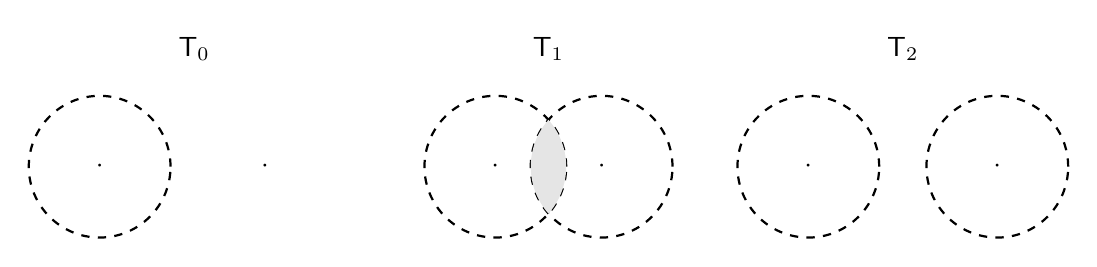
\begin{tikzpicture}[scale = 0.3]
			\draw[black,thick,dashed] (4,0) circle (3); 
			\node at (4,0) {$\cdot$};
			\node at (8,5) {$\mathsf{T}_0$};
			\node at (11,0) {$\cdot$};
			
			\draw[black,thick,dashed] (20.75,0) circle (3);
			\node at (20.75,0) {$\cdot$};
			\node at (23, 5) {$\mathsf{T}_1$};
			\draw[black,thick,dashed] (25.25,0) circle (3);
			\node at (25.25,0) {$\cdot$};
			
			\begin{scope}
				\clip (20.75,0) circle (3);
				\fill[black!10] (25.25,0) circle (3);
			\end{scope}
			
			\draw[black,thick,dashed] (34,0) circle (3);
			\node at (34,0) {$\cdot$};
			\node at (38,5) {$\mathsf{T}_2$};
			\draw[black,thick,dashed] (42,0) circle (3);
			\node at (42,0) {$\cdot$};
		\end{tikzpicture}
	\end{center}
	
	\begin{mathSection}
		\begin{defn}
			A topology for $X$ is \textbf{Kolmogorov} (or $\mathsf{T}_0$) if for every two elements $x_1, x_2 \in X$ there exists a verifiable set $U \in \mathsf{T}_X$ containing one element but not the other. That is: either $x_1 \in U$ while $x_2 \notin U$ or $x_1 \notin U$ while $x_2 \in U$.
		\end{defn}
		\begin{defn}
			A topology for $X$ is \textbf{Fr\'echet} (or $\mathsf{T}_1$) if for every two elements $x_1, x_2 \in X$ there exist two, not necessarily disjoint, verifiable sets $U_1, U_2 \in \mathsf{T}_X$ each containing only one element. That is: $x_1 
			\in U_1$ and $x_2 \in U_2$.
		\end{defn}
		\begin{defn}
			A topology for $X$ is \textbf{Hausdorff} (or $\mathsf{T}_2$) if for every two elements $x_1, x_2 \in X$ there exist two disjoint verifiable sets $U_1, U_2 \in \mathsf{T}_X$ each containing one element. That is: $U_1 \cap U_2 = \emptyset$, $x_1 
			\in U_1$ and $x_2 \in U_2$.
		\end{defn}
		\begin{remark}
			Note that $\mathsf{T}_2$ implies $\mathsf{T}_1$ which in turn implies $\mathsf{T}_0$.
		\end{remark}
		
	\end{mathSection}
	
	How do these properties relate to experimental domains? Consider two possibilities for a domain, for example \statement{that is a cat} and \statement{that is a swan}. We can always find a verifiable statement, such as \statement{that animal has feathers}, that we can use to distinguish one possibility from the other. This means that, given two different possibilities, we can always find a verifiable set that contains one and not the other: the natural topology for any set of possibilities is always $\mathsf{T}_0$.
	
	Now suppose two possibilities are approximately verifiable as we defined in Definition \ref{pm-vs-defApproximatelyVerifiable}. For example, \statement{the mass of the photon is exactly 0 eV} or \statement{the mass of the photon is exactly $10^{-20}$ eV}. We can find two verifiable statements \statement{the mass of the photon is less than $10^{-25}$ eV} and \statement{the mass of the photon is more than $10^{-25}$ eV} each compatible with only one possibility. This means that, given two approximately verifiable possibilities, we can find two verifiable sets each containing only one possibility: if all possibilities are approximately verifiable then the natural topology is $\mathsf{T}_1$.
	
	Now suppose two possibilities are experimentally distinguishable as we defined in Definition \ref{pm-vs-defExperimentallyDistinguishable}. Then, by \ref{pm-vs-experimentallyDistinguishableIsDisjointApproximation}, we can find two disjoint approximations. In the example before, the two verifiable statements were in fact incompatible. This means that, given two approximately verifiable possibilities, we can find two disjoint verifiable sets each containing only one possibility: if all possibilities are experimentally distinguishable then the natural topology is $\mathsf{T}_2$.
	
	\begin{mathSection}
		\begin{prop}
			The natural topology of a set of possibilities is Kolmogorov (or $\mathsf{T}_0$).
		\end{prop}
		\begin{proof}
			Let $X$ be the set of possibilities for an experimental domain $\edomain$. Let $x_1, x_2 \in X$ be two distinct possibilities. Each of them can be expressed as a minterm of a basis $\basis \subseteq \edomain$. Since the two possibilities are distinct, there must exist a verifiable statement $\stmt[e] \in \basis$ that appears negated in one conjunction but not the other. That is, $\stmt[e]$ is compatible with only one possibility. Since the verifiable set associated with a verifiable statement contains only the possibilities compatible with said statement, the verifiable set of $\stmt[e]$ either contains $x_1$ or $x_2$ but not both. The topology is therefore Kolmogorov (or $\mathsf{T}_0$).
		\end{proof}
		\begin{prop}
			The natural topology of a set of possibilities is Fr\'echet (or $\mathsf{T}_1$) if and only if all possibilities are approximately verifiable.
		\end{prop}
		\begin{proof}
			% TODO: Could be shorten since it is sufficient to just prove one side (I.e. given x,y in X, find U containing x but not y. No need to find another set for y. Because the points were arbitrary there is no loss of generality).
			Suppose all possibilities in $X$ for an experimental domain $\edomain_X$ are approximately verifiable. Let $x_1, x_2 \in X$ be two possibilities, then we can find two sequences of verifiable statements $\{\stmt_i^1\}_{i=1}^\infty, \{\stmt_j^2\}_{j=1}^\infty \in \edomain_X$ such that $x_1=\bigAND\limits_{i=1}^\infty \stmt_i^1$ and $x_2=\bigAND\limits_{j=1}^\infty \stmt_j^2$. We can assume the sequences are monotone with respect to narrowness, that is $\stmt_{i+1}^1 \narrower \stmt_i^1$, as we can always create a monotone sequence from one that is not by taking the sequence of finite conjunction, that is $\hat{\stmt}_k^1=\bigAND\limits_{i=1}^k \stmt_i^1$. If $x_1 \neq x_2$, then $x_1 \AND x_2 \equiv \impossibility$ since different possibilities are incompatible. Therefore we must have $x_1 \AND \stmt_j^2 \equiv \impossibility$ and $\stmt_i^1 \AND x_2 \equiv \impossibility$ from some $i,j \geq 1$ or the limits would not be incompatible. In terms of verifiable sets we have $x_2 \notin U(\stmt_i^1)$ and $x_1 \notin U(\stmt_j^2)$. For any two distinct possibilities we can find two verifiable sets each containing one: the natural topology is $\mathsf{T}_1$.
			
			Conversely, suppose the natural topology $\mathsf{T}_X$ for the possibilities $X$ for an experimental domain $\edomain_X$ is $\mathsf{T}_1$. Let $x \in X$ be a possibility. Consider the collection, not necessarily countable, of all verifiable sets $\{U_i\}_{i \in I} \subset \mathsf{T}_X$ such that they contain $x$. Consider their intersection $U_x = \bigcap\limits_{i \in I} U_i$. It will contain $x$ since all $U_i$ contain $x$. It will not contain anything else: since the topology is $\mathsf{T}_1$, for every other possibility $\hat{x}$ there is always an open set $U_i$ that does not contain it. Therefore $U_x = \{x\}$. Because the natural topology is second countable, we can find a countable basis $\basis$ and rewrite the arbitrary intersection into $\{x\} = \bigcap\limits_{i=1}^\infty V_i$ a countable intersection of elements $V_i \in \basis$ of the basis. Let $\{\stmt_i\}_{i=1}^\infty$ be the sequence of verifiable statements such that $U(\stmt_i) = V_i$ for every $i$. Then $x=\bigAND\limits_{i=1}^\infty \stmt_i$ which means $x$ is approximately verifiable.
			
		\end{proof}
		\begin{prop}
			The natural topology of a set of possibilities is Hausdorff (or $\mathsf{T}_2$) if and only if all possibilities are pairwise experimentally distinguishable.
		\end{prop}
		\begin{proof}
			Suppose all possibilities in $X$ for an experimental domain $\edomain_X$ are pairwise experimentally distinguishable. Then, by \ref{pm-vs-experimentallyDistinguishableIsDisjointApproximation}, given two possibilities $x_1, x_2 \in X$ we can find two verifiable statements $\stmt_1, \stmt_2 \in \edomain_X$ such that $\stmt_1 \ncomp \stmt_2$, $x_1 \narrower \stmt_1$ and $x_2 \narrower \stmt_2$. In terms of verifiable sets we have $U(\stmt_1) \cap U(\stmt_2) = \emptyset$, $x_1 \in U(\stmt_1)$ and $x_2 \in U(\stmt_2)$. The topology is $\mathsf{T}_2$.
			
			Conversely, suppose the natural topology $\mathsf{T}_X$ for the possibilities $X$ for an experimental domain $\edomain_X$ is $\mathsf{T}_2$. Given two possibilities $x_1, x_2 \in X$ we can find two verifiable sets $U_1, U_2 \in \mathsf{T}_X$ such that $U_1 \cap U_2 = \emptyset$, $x_1 \in U_1$ and $x_2 \in U_2$. Since $U_1, U_2 \in \mathsf{T}_X$, we can find two corresponding verifiable statements $\stmt_1, \stmt_2 \in \edomain_X$ such that $U(\stmt_1) = U_1$ and $U(\stmt_2) = U_2$. We have $\stmt_1 \ncomp \stmt_2$, $x_1 \narrower \stmt_1$ and $x_2 \narrower \stmt_2$ and by \ref{pm-vs-experimentallyDistinguishableIsDisjointApproximation} the possibilities are pairwise experimentally distinguishable.
		\end{proof}
	\end{mathSection}
	
	\section{Sigma-algebras}
	
	In the same way that experimental domains find a natural mathematical representation as topological spaces, theoretical domains find a natural mathematical representation in $\sigma$-algebras. The main result of this section is that a theoretical domain provides a natural $\sigma$-algebra on its possibilities.
	
	Like topologies, $\sigma$-algebras are fundamental in mathematics as they allow us to construct measures (i.e.~assigning sizes to sets), limits for sequences of sets and probability spaces. It is again fitting that theoretical domains are associated to such a fundamental mathematical structure.
	
	Let's first review what a $\sigma$-algebra is. The general idea is that we have a set $X$ of elements which we call points, and we have a collection of subsets of $X$ such that it is closed under complement and countable union, contains the empty set and contains the whole set $X$. For example, suppose $X = \{1,2,3\}$ then  $\{\{\},\{1\},\{1,2,3\}\}$ is not a $\sigma$-algebra while $\{\{\},\{1\}, \{2,3\},\{1,2,3\}\}$ is. The first one is missing the complement of $\{1\}$.
	
	\begin{mathSection}
		\begin{defn}
			Let $X$ be a set. A \textbf{$\sigma$-algebra} on $X$ is a collection $\Sigma_X$ of subsets of $X$ closed under complement and countable union such that it contains $X$.
		\end{defn}
	\end{mathSection}
	
	Note that $\sigma$-algebras are also closed under countable intersections, since these can be expressed in terms of complements and countable unions.
	
	In the previous section we saw how each verifiable statement can be expressed as the conjunction of a set of possibilities, how the operations on statements can be expressed as operations on the verifiable sets and how all the verifiable sets form a topology. The same is true for theoretical statements, with the only difference being that we will end up with a collection of sets that is closed under complement and countable union since the theoretical domain is closed under negation and countable disjunction.
	
	\begin{mathSection}
		
		\begin{defn}
			Let $\tdomain$ be a theoretical domain and $X$ its possibilities. We define the map $A : \tdomain \rightarrow 2^X$ that for each theoretical statement $\stmt \in \tdomain$ returns the set of possibilities compatible with it. That is, $A(\stmt)\equiv\{ x \in X \, | \, x \comp \stmt\}$. We call $A(\stmt)$ the \textbf{theoretical set} of possibilities associated with $\stmt$
		\end{defn}
		
		\begin{prop}
			Let $X$ be the set of possibilities for a theoretical domain $\tdomain$. $X$ has a natural $\sigma$-algebra given by the collection of all theoretical sets $\Sigma_X=A(\tdomain)$.
		\end{prop}
		
		\begin{proof}
			The theoretical sets for the certainty and the impossibility correspond to the full set and empty set respectively. Formally, $A(\certainty) = \{ x \in X \, | \, x \comp \certainty\} = X$ while $A(\impossibility) = \{ x \in X \, | \, x \comp \impossibility\} = \emptyset$. Therefore $X, \emptyset \in A(\tdomain)$ since $\certainty, \impossibility \in \tdomain$.
			
			The complement of a theoretical set corresponds to the theoretical set of the negation and therefore it is a theoretical set. Formally, $A(\stmt)^C = \{ x \in X \, | \, x \ncomp \stmt\} =  \{ x \in X \, | \, x \comp \NOT\stmt\} = A(\NOT\stmt)$.
			
			The countable union of verifiable sets corresponds to the verifiable set of the countable disjunction and therefore it is a theoretical set. Formally, $A(\stmt_1\OR\stmt_2) = \{ x \in X \, | \, x \comp \stmt_1\OR\stmt_2\} =  \{ x \in X \, | \, x \comp \stmt_1 \, or \, x \comp \stmt_2\} = \{ x \in X \, | \, x \comp \stmt_1\} \cup \{ x \in X \, | \, x \comp \stmt_2\} = A(\stmt_1) \cup A(\stmt_2)$. This generalizes to countable disjunctions.
			
			The collection $\Sigma_X=A(\tdomain)$ is therefore a $\sigma$-algebra by definition since it satisfies all its properties.
		\end{proof}
	\end{mathSection}
	
	There is also a special link between topologies and $\sigma$-algebras. As one may want to construct measures and probability spaces on topological spaces, there is a standard way to construct a $\sigma$-algebra from a topology. This object, called Borel algebra, is the smallest $\sigma$-algebra that contains all verifiable sets defined by the topology. The $\sigma$-algebra defined by a theoretical domain is none other than the Borel algebra of the topology defined by the corresponding experimental domain.
	
	\begin{mathSection}
		
		\begin{defn}
			Let $(X, \mathsf{T})$ be a topological space. Its \textbf{Borel algebra} is the collection $\Sigma_X$ of subsets of $X$ generated by countable union, countable intersection and complement from the verifiable sets.
		\end{defn}
		
		\begin{prop}
			The natural $\sigma$-algebra for a set of possibilities is the Borel algebra of its natural topology.
		\end{prop}
		
		\begin{proof}
			Since the theoretical domain can be generated by a basis of the experimental domain, the natural $\sigma$-algebra can be generated by a sub-basis of the natural topology. This means that it is also generated by countable union, countable intersection and negation from the verifiable sets of the natural topology.
		\end{proof}
	\end{mathSection}
	
	This fundamental link between experimental domains and topology on one side and theoretical domains and $\sigma$-algebra on the other is important for multiple reasons.
	
	From a practical standpoint, it guarantees that these mathematical tools can always be used in science. Since experimental and theoretical domains are general constructs, any branch of scientific investigation can use techniques and results from topology and $\sigma$-algebras for calculations or for characterizing the domain at hand.
	
	From a conceptual standpoint it provides a Rosetta stone, i.e a way to translate, between the mathematical concepts and the scientific ones. It gives a precise scientific meaning to the mathematical tools and everything built on top of them. Every single step in a calculation, every single argument in a proof can be given a clear, and possibly insightful, physical meaning. It grounds the abstract mathematical language in more concrete scientific objects. This in turn helps clarify the science described by common mathematical tools, unearthing possible hidden assumptions or simplifications about the physical systems being studied.
	
	This connection explains why these mathematical tools have found such successful application in the physical sciences.
	
	\section{Decidable domains}
	
	We conclude this chapter by analyzing decidable domains, those for which we can experimentally test both the truth and the falsehood of all statements. For example, the domain for animal identification and the domain for the amount of money in my pocket can be considered decidable as we can typically tell experimentally whether \statement{this animal has whiskers} or not, or whether \statement{there is more than one dollar and fifty cents in my pocket} or not.
	
	Decidable domains have special characteristics and are easier to study. Since we can verify the negation, any theoretical statement is also verifiable. And since all theoretical statements are verifiable, so are the possibilities. That is, we can verify that \statement{this animal is a cat} and that \statement{there are two dollars and thirty cents in my pocket}. As all statements can be expressed as a disjunction of possibilities, the possibilities themselves form a countable basis. For example, \statement{there is more than one dollars and fifty cents in my pocket} can be expressed as the disjunction of the appropriate statements of the form \statement{there are x dollars and y cents in my pocket}.
	
	\begin{mathSection}
		\begin{defn}
			An experimental domain $\edomain_X$ is \textbf{decidable} if all statements in the domain are decidable. Formally, for every $\stmt \in \edomain_X$ we have $\NOT\stmt \in \edomain_X$.
		\end{defn}
		
		\begin{prop}\label{pm-vs-decidableDomainProperties}
			Let $\edomain_X$ be an experimental domain. The following are equivalent:
			\begin{enumerate}
				\item the experimental domain is decidable
				\item the experimental domain and its theoretical domain coincide
				\item all possibilities are verifiable
				\item the possibilities form a countable basis.
			\end{enumerate}
		\end{prop}
		
		\begin{proof}
			To prove 2 from 1, suppose $\edomain_X$ is a decidable experimental domain. As $\edomain_X$ is decidable, it is already closed under negation and therefore all statements in its theoretical domain $\tdomain_X$ are already in $\edomain_X$.
			
			To prove 3 from 2, suppose $\edomain_X$ coincides with its theoretical domain $\tdomain_X$. As each possibility is a theoretical statement, it is also a verifiable statement.
			
			To prove 4 from 3, suppose the possibilities are verifiable. Note that the possibilities can generate all other statements through disjunction. To show $X$ is countable, consider a countable basis $\basis \subseteq \edomain_X$. Because the possibilities are verifiable statements, they can be generated from $\basis$ by finite conjunction and countable disjunction. Moreover, since the possibilities are the narrowest statements that are not impossible, they can be generated from $\basis$ using finite conjunction only. Since $\basis$ is countable and $X$ is generated by $\basis$ through finite conjunction, $X$ can be at most countable. Therefore $X$ is a countable basis.
			
			To prove 1 from 4, suppose the possibilities $X$ form a countable basis. Then each possibility is verifiable and so is their countable union. The negation of a verifiable statement can be expressed as the countable union of possibilities, and is therefore verifiable. All statements in the experimental domain are decidable and therefore the domain is decidable.
		\end{proof}
	\end{mathSection}
	
	As the possibilities for a decidable domain must form a countable basis, their cardinality can't be greater than countable. That is: only domains that are non-decidable can have possibilities with cardinality of the continuum. In this sense they are more constrained and simpler to study.
	
	Mathematically, the natural topology corresponds to the discrete topology: the one for which any subsets of the possibilities is a verifiable set. That is, the topology is simply the set of all possible sets of possibilities. The cardinality of the possibility is therefore enough to determine the topology of the space, which means that one number is enough to characterize the space.
	
	\begin{mathSection}
		\begin{defn}
			A topology $\mathsf{T}_X$ on a set $X$ is called \textbf{discrete} if it contains every subset of $X$.
		\end{defn}
		
		\begin{thrm}[Decidability is discreteness]\label{pm-vs-decidabilityIsDiscreteness}
			The natural topology of the possibilities $X$ for a domain $\edomain_X$ is discrete if and only if the domain is decidable.
		\end{thrm}
		\begin{proof}
			Suppose $\edomain_X$ is decidable. Let $U \subseteq X$ be a subset of possibilities. The statement $\stmt = \bigOR\limits_{x \in U} x$ is generated from $X$ through countable disjunction. Since $\edomain_X$ is decidable, $X$ is a countable basis and $\stmt$ is verifiable. Therefore $U$ is a verifiable set and it is contained in the natural topology. The natural topology of $X$ is discrete by definition.
			
			Now suppose $\edomain_X$ is such that the natural topology for its possibilities $X$ is discrete. Let $\stmt = \bigOR\limits_{x \in U} x$ be a statement. Since the topology is discrete, $U$ is part of the topology and $\stmt$ is verifiable. Consider its negation $\NOT\stmt = \bigOR\limits_{x \in U^C} x$. Since the topology is discrete, $U^C$ is also part of the topology and $\NOT\stmt$ is verifiable. This means $\stmt$ is decidable. Since every statement in $\edomain_X$ is decidable, the domain is decidable.
		\end{proof}
		
	\end{mathSection}
	
	Note, though, that discrete does not imply finite or vice-versa. The domain for extra-terrestrial life is finite but is not decidable as we cannot verify that \statement{there is no extra-terrestrial life}. The domain for the amount of money in my pocket, instead, is decidable but not necessarily finite as I could potentially have an arbitrarily large amount.
	
	\section{Summary}
	
	In this first chapter we have laid down the foundations for our general mathematical theory of experimental science. We have seen how it is grounded in the logic of verifiable statements, which is more limited than the logic of pure statements as it has to deal with the practical constraints introduced by the termination of the tests.
	
	
	\begin{center}
		\begin{tikzpicture}
			\node[draw, minimum width=10.5cm, minimum height=5.3cm, rounded corners=5mm] (bdx) {};
			\node[align=center, below] at ([yshift=-1mm]bdx.north) {\textbf{Theoretical statements} \\statements associated with an experimental test};
			\node[align=center, above left] at (bdx.157) {$\tdomain_X$};
			\node[align=center, above] at (bdx.north) {\textbf{Statements} ($\AND$ $\OR$ $\NOT$ $\impossibility$ $\certainty$)};
			
			\node[ellipse, draw, minimum width=5cm, minimum height=3.5cm, align=center, inner xsep=-2mm] (vs) at ([xshift=-1.85cm, yshift=-5mm]bdx) {\textbf{Verifiable statements}\\[1mm]
				if true, test always\\
				succeeds};
			\node[align=center, above left] at (vs.145) {$\edomain_X$};
			\node[ellipse, draw, minimum width=4.2cm, minimum height=2.7cm, align=center,inner xsep=0mm] (poss) at ([xshift=2.25cm,yshift=-7mm]bdx) {\textbf{Possibilities}\\[1mm]
				experimentally\\
				distinguishable\\
				cases
			};
			\node[align=center, above right] at (poss.90-55) {$X$};
			
			\node[draw, minimum width=4.8cm, minimum height=3cm, rounded corners=5mm, anchor=north west] (sx) at ([yshift=-5mm]bdx.south west) {};
			\node[align=center, above] at ([xshift=-3mm,yshift=0.5mm]sx.-115) {\textbf{Borel sets}};
			\node[align=center, above left] at (sx.155) {$\Sigma_X$};
			
			\node[ellipse, minimum width=3cm, minimum height=2cm, draw] (os) at ([xshift=3mm,yshift=1mm]sx) {\textbf{Open sets}};
			\node[align=center, above left] at (os.150) {$\mathsf{T}_X$};
			\node[ellipse, minimum width=2.8cm, minimum height=1.8cm, draw] (point) at([yshift=-1mm]os-|poss)  {\textbf{Points}};
			\node[align=center, below=3.6cm] at (bdx.south) {\textbf{Sets} ($\cup$ $\cap$ $\complement$ $X$ $\emptyset$)};
			\node[align=center, above right] at (point.90-55) {$X$};
			
			\coordinate (z) at (bdx.south);
			\draw[stealth'-stealth'] (sx.130)--(z-|sx.130);
			\draw[stealth'-stealth'] (vs.south) to (os.90);
			\draw[stealth'-stealth'] (poss.south) to (point);
			\draw[stealth'-stealth'] ([xshift=2mm]sx.east)--+(8mm,0);
			
			\draw[gray, dashed, thick] (-6,-2.75)--+(11.5,0);
		\end{tikzpicture}
	\end{center}
	
	
	We saw that we can group verifiable statements into experimental domains which must have a countable basis to allow us to test any statement within an indefinite amount of time. We saw how to construct theoretical domains to find all the theoretical statements that can be associated to an experimental test. And we saw how the possibilities are those statements that, if true, give a complete prediction for all statements in the domain.
	
	We have seen that, because of the disjunctive normal form, each verifiable and theoretical statement is equivalent to a set of possibilities and how logic operations and relationships become set operations and relationships. As such, the experimental and theoretical domains respectively provide a natural topology and $\sigma$-algebra for the possibilities.
	
	What we have ended up with is a conceptual framework that captures the necessary elements of scientific practice and codifies them into a symbolic representation with a well defined meaning. There is no guesswork as to what the points of our spaces are: they are the possibilities, statements that provide a complete description for the domain. We do not have to provide an ``interpretation" as to what the sets of a topology represent: they correspond to verifiable statements. All the objects have a clear definition and meaning from the start, we know which ones are necessary and to what extent they are physical or idealized. This will provide a much more solid foundation to the rest of the work, which will ultimately allow us to understand much better the fundamental physical theories and the connections between them and to other areas of scientific thought.
	
	
	
	\newpage
	
	\section{Reference sheet}
	
	\begin{tabular}{p{0.2\textwidth} p{0.3\textwidth} p{0.5\textwidth}}
		& Name & Meaning  \\ 
		\hline 
		$\Bool$  & Boolean domain & the set of possible truth values \\ 
		&  & i.e.~$\Bool = \{\TRUE, \FALSE\}$ \\ 
		\hline 
		$\logCtx$ & logical context & a set of statements with well defined logical relationships \\ 
		\hline 
		$\stmt \in \logCtx$ & statement & an assertion with a well defined truth value \\ 
		\hline 
		$\truth : \logCtx \to \Bool$ & the truth function & returns whether a statement is true or not  \\ 
		\hline 
		$\pAss \subseteq \Bool^\logCtx$& possible assignments & the logically consistent truth value combinations that can be assigned to the statements \\ 
		\hline 
		$\certainty$ & certainty & a statement that can only be true (i.e.~it is true in all possible assignments) \\ 
		\hline 
		$\impossibility$ & impossibility & a statement that can never be true (i.e.~it is false in all possible assignments) \\ 
		\hline 
		& contingent statement & a statement that can be either true or false depending on the possible assignment \\ 
		\hline 
		$\NOT \stmt$ & negation (logical NOT) & the statement whose truth value is always opposite \\ 
		\hline 
		$\stmt_1 \AND \stmt_2$ & conjunction (logical AND) & the statement that is true only if all statements are true \\ 
		\hline 
		$\stmt_1 \OR \stmt_2$ & disjunction (logical OR) & the statement that is true if any of the statements is true \\ 
		\hline 
		$\stmt_1 \equiv \stmt_2$ & equivalence & whether each statement is a logical consequence of the other (i.e.~they must have the same value in every possible assignment) \\ 
		\hline 
		$\stmt_1 \narrower \stmt_2$ & narrower than & whether the first statement is more specific than the second (i.e.~in every possible assignment, if the first is true than the second must be also true) \\ 
		\hline 
		$\stmt_1 \broader \stmt_2$ & broader than & whether the second statement is narrower than the first \\ 
		\hline 
		$\stmt_1 \comp \stmt_2$ & compatibility & whether both statement can be true at the same time (i.e.~there is a possible assignment in which they are both true) \\
		\hline 
		$\stmt_1 \indep \stmt_2$ & independence & whether both statement can be true at the same time (i.e.~there is a possible assignment for each combination of their possible truths) \\
		\hline 
		& minterm & a conjunction where each statement appears once, either negated or not \\
		\hline 
		$\stmt \in \vstmtSet$ & verifiable statement & a statement that can be validated experimentally\\ 
		\hline 
		$\edomain$ & experimental domain & a set of verifiable statements that can be tested in an indefinite amount of time (i.e.~a set of statements closed under finite conjunction and countable disjunction, that precisely contains the certainty, the impossibility and a set of verifiable statements generated by a countable basis) \\ 
		\hline 
		$\basis \in \edomain$ & basis & a set of verifiable statements from which all others can be constructed\\ 
		
	\end{tabular} 
	
	\newpage
	
	\begin{tabular}{p{0.2\textwidth} p{0.3\textwidth} p{0.5\textwidth}}
		& Name & Meaning  \\ 
		\hline 
		$\tdomain$ & theoretical domain & the set of all statements constructed from an experimental domain that can be associated with an experimental test\\ 
		\hline 
		& approximately verifiable & when a statement is not verifiable but is the limit of a sequence of statements that are\\ 
		\hline 
		$X$ & possibilities of a domain & those statements that, if true, determine the value of all verifiable statements of a domain\\ 
		\hline 
		$\estPoss$ & established possibility & a possibility for which at least a verifiable statement is true (i.e.~it can be established experimentally)\\ 
		\hline 
		$\resPoss$ & residual possibility & if it exists, the possibility for which all verifiable statements are false (i.e.~the remaining case that cannot be established experimentally)\\ 
		
	\end{tabular} 
	
